\documentclass[11pt,openany,oneside,letterpaper]{book_tesis}
\usepackage[spanish]{babel}
%\usepackage[utf8]{inputenc}
\usepackage{fontspec}			% Necesario para XeLaTeX o LuaLaTeX
\usepackage{setspace}           % Interlineado
\usepackage{titletoc}			% Formato del indice
\usepackage{titlesec}			% Formato del indice
\usepackage[left=2.54cm, right=2.54cm, top=2.54cm, bottom=2.54cm]{geometry}

\usepackage{graphicx}  % Para insertar imágenes
\usepackage{caption}   % Para personalizar leyendas
\usepackage{float}     % Para control de posicionamiento de figuras
\usepackage{booktabs}   % Para líneas horizontales en
\usepackage{array}      % Para personalizar alineación en columnas
\usepackage{longtable} % Paquete para tablas largas
\usepackage{multirow} % para unión de filas en las tablas

\usepackage{changepage} % Para ajustar márgenes

\usepackage{amssymb}
\usepackage{amsfonts}
\usepackage{amsmath}
\usepackage[backend=biber, style=apa]{biblatex} % Para usar bibliografia
\usepackage{csquotes}
\usepackage{enumitem}			% para las listas 
\usepackage[nopatch=item]{microtype}		% Para que no salga error de polyglossia
\usepackage{lipsum} % Carga el paquete lipsum
\usepackage{microtype}
\usepackage{hyperref} % Para enlaces a los capitulos secciones en el indice

% \usepackage{showframe}                % Para ver lineas de margenes

\addbibresource{parte_final/bibliografia.bib}

\setmainfont{georgia} 			% Configura la fuente principal como Georgia

\setlength{\parskip}{0.1mm}           % Espacio entre párrafos
\setlength{\parindent}{36.1315pt}     % Indentación de los párrafos
\setlength{\baselineskip}{0em} % Ajusta el espacio entre líneas

\pagestyle{myheadings}

% Cambiar "Cuadro" a "Tabla"
\addto\captionsspanish{\renewcommand{\tablename}{Tabla}}
% Cambiar "Índice de Cuadros" a "Índice de Tablas"
\addto\captionsspanish{\renewcommand{\listtablename}{ÍNDICE DE TABLAS}}
% Cambiar "Índice de figuras" a "ÍNDICE DE FIGURAS"
\addto\captionsspanish{\renewcommand{\listfigurename}{ÍNDICE DE FIGURAS}}

\assignpagestyle{\chapter}{empty} % Para que las hojas de los capítulos no sean numeradas

% Ajustar el espaciado vertical entre los capítulos en el índice
\titlecontents{chapter}[0pt]{\addvspace{1pt}\bfseries}{\thecontentslabel.\hspace{1.6em}}{}{\titlerule*[0.5pc]{.}\contentspage}
\titlecontents{section}[0pt]{}{\thecontentslabel.\hspace{1em}}{}{\titlerule*[0.5pc]{.}\contentspage}
\titlecontents{subsection}[28pt]{}{\thecontentslabel.\hspace{1em}}{}{\titlerule*[0.5pc]{.}\contentspage}

% Cambiar los títulos de los capítulos a mayúsculas
% \titleformat{\chapter}[display]
%{\normalfont\fontsize{13pt}{42pt}\selectfont\bfseries}{\MakeUppercase{\chaptertitlename}\ \thechapter}{-110pt}{\fontsize{13pt}{70pt}\selectfont}

\titleformat{\chapter}
{\normalfont\fontsize{13pt}{60pt}\selectfont\bfseries}{\thechapter}{24pt}{\fontsize{13pt}{0pt}\selectfont}

\titleformat{\section}{\bfseries\normalsize}{\thesection.}{16pt}{}
\titleformat{\subsection}{\bfseries\normalsize}{\thesubsection.}{9pt}{}

\titlespacing*{\chapter}{0pt}{*0}{0pt}
\titlespacing*{\section}{0pt}{*0}{0pt}
\titlespacing*{\subsection}{0pt}{*0}{0pt}

% Definir un nuevo estilo de numeración para los capítulos
% \renewcommand{\thechapter}{\Roman{chapter}}

% Configuración de hyperref para desactivar colores y cuadros
\hypersetup{
	colorlinks=false, % Desactiva el color de los enlaces
	pdfborder={0 0 0}, % Desactiva los cuadros alrededor de los enlaces
}

\captionsetup[figure]{
	margin={1.27cm,0cm},
	justification=RaggedRight, % Alineación a la izquierda
	singlelinecheck=false,     % Permite leyendas de múltiples líneas
	labelfont=bf,              % Fuente de etiqueta en negrita
	textfont=it,         	% Fuente en cursiva para texto
	labelsep=newline,           % Separador es un punto
}

\captionsetup[table]{
	margin={1.27cm,0cm},
	labelfont=bf,
	labelsep=newline,
	justification=RaggedRight,
	singlelinecheck=false,     % Permite leyendas de múltiples líneas
	textfont=it,      % Texto de la leyenda en cursiva
	% position=top,     % Leyenda arriba de la tabla
	% skip=0pt          % Sin espacio entre la leyenda y la tabla
}

\captionsetup[longtable]{
	margin={1.27cm,0cm},
	labelfont=bf,
	labelsep=newline,
	justification=RaggedRight,
	singlelinecheck=false,     % Permite leyendas de múltiples líneas
	textfont=it,      % Texto de la leyenda en cursiva
	% position=top,     % Leyenda arriba de la tabla
	skip=17pt          % Sin espacio entre la leyenda y la tabla
}

\makeatletter
\renewcommand\listoffigures{%
	\chapter*{\hfill\bfseries\normalsize ÍNDICE DE FIGURAS\hfill} % Título centrado
	\addcontentsline{toc}{chapter}{\listfigurename}%
	\noindent\hspace{0.6cm}\textbf{Fig.} \hfill \textbf{Descripción} \hfill \textbf{Pag.} \hfill % Encabezados
	\par\vspace{-0.2cm} % Espacio entre encabezados y el listado
	\@starttoc{lof}%
}
\makeatother

% Modificar el formato del índice de tablas
\makeatletter
\renewcommand\listoftables{%
	\chapter*{\hfill\bfseries\normalsize ÍNDICE DE TABLAS\hfill} % Título centrado
	\addcontentsline{toc}{chapter}{\listtablename}%
	\noindent\hspace{0.6cm}\textbf{Tabla} \hfill \textbf{Descripción} \hfill \textbf{Pag.} \hfill % Encabezados
	\par\vspace{-0.2cm} % Espacio entre encabezados y el listado
	\@starttoc{lot}%
}
\makeatother

\begin{document}
	\spacing{2}                     % Interlineado
	\frontmatter
	\pagenumbering{gobble} % Eliminar numeración de página del índice
	\begin{titlepage}
	\begin{center}
		{\textbf{UNIVERSIDAD MAYOR DE SAN ANDRÉS}}\\
		{\textbf{FACULTAD DE CIENCIAS PURAS Y NATURALES}}\\
		{\textbf{CARRERA DE INFORMÁTICA}}\\
		\vspace{5mm}
		\begin{figure}[h]
			\centering
			
\includegraphics[scale=1.09]{imagenes/Logo_UMSA.png}
		\end{figure}
		\vspace{3mm}
		{\textbf{PROYECTO DE GRADO}}\\
		
		{\textbf{SOFTWARE DE LOGÍSTICA Y GESTIÓN DE BUSES PARA TRANSPORTE DE PASAJEROS Y ENVÍO DE ENCOMIENDAS.\\
		CASO: EMPRESA DE TRANSPORTES CALI INTERNACIONAL}}\\
		{Proyecto de Grado para obtener el Título de Licenciatura en Informática}\\
		Mención: Ingeniería de Sistemas Informáticos\\
		
		\textbf{POSTULANTE:} BLADIMIR WILSON RAMOS ESCOBAR\\
		\textbf{TUTOR:} Ph. D. FRANZ CUEVAS QUIROZ\\
		\textbf{NUESTRA SEÑORA DE LA PAZ – BOLIVIA}\\
		\textbf{2025}\\
	\end{center}
\end{titlepage}
	\thispagestyle{empty}
	\sloppy
	% Dedicatoria
	%% Contenido del resumen
\thispagestyle{plain}

\vspace*{4cm} % Ajusta este espacio vertical según necesites

\begin{flushright}
	{\bfseries\fontsize{13pt}{16pt}\selectfont DEDICATORIA}
\end{flushright}

%\vspace{2cm} % Espacio entre el título y el texto

\begin{flushright}
	\textit{A mis padres, por ser el pilar fundamental de mi vida y por enseñarme con su ejemplo el valor del esfuerzo y la perseverancia. En especial, a mi querida madre Celia (+), que desde el cielo me acompaña e ilumina mi camino; por ser la única que confiaba en mí, su amor infinito sigue guiando cada uno de mis pasos.}
	
	\vspace{0.2cm}
	
	\textit{A mi amada esposa Rosmery, por su paciencia, apoyo incondicional y por creer en mí incluso en los momentos más difíciles.}
	
	\vspace{0.2cm}
	
	\textit{Y a mi cuatro patitas Duke, mi leal compañero, cuyo cariño y alegría hicieron más llevaderos los días de estudio.}
	
	\vspace{0.2cm}
	
	\textit{A todos ustedes, gracias por ser mi inspiración y mi fuerza.}
\end{flushright}
	% Agradecimientos
	%\chapter*{Agradecimientos} 

	\renewcommand{\contentsname}{\hfill\bfseries\normalsize CONTENIDO\hfill}
	\tableofcontents
	\thispagestyle{empty}
	\addtocontents{toc}{~\hfill\textbf{Pág.}\par}
	
	% Índice de Figuras
	% \listoffigures
	
	
	% Índice de Tablas
	% \listoftables
	
	\mainmatter
	% Introduccción
	\setcounter{page}{1}
	\chapter{INTRODUCCIÓN}

	\vspace{10pt}

	Los avances actuales de la informática y la difusión global de la Internet han cambiado la manera en que se desarrollan las actividades de la sociedad en los ámbitos de la comunicación, la calidad de vida y el comercio. Internet ofrece nuevas alternativas de negocio ya que esta nos permite llegar a una audiencia masiva y a un gran número de posibles clientes; podemos ofrecer nuestros servicios a un mercado mucho mayor porque el tiempo y la distancia dejan de ser obstáculos \parencite{anormaliza2009implementacion}.
	
	% 16En esta era de la transformación digital, las Tecnologías de la Información y Comunicación (TICs) desempeñan un rol esencial al ser una combinación de servicios, redes, software y dispositivos completamente integrados. Las TICs se integran en un sistema de información interconectado y complementan un entorno económico y social, con el objetivo de mejorar constantemente las operaciones empresariales y la calidad de vida de los individuos. Las empresas y organizaciones utilizan las TICs con el objetivo principal de mejorar y acelerar los procesos internos, facilitar la toma de decisiones y obtener una ventaja competitiva notable en el mercado. Las organizaciones pueden mejorar su eficiencia y efectividad, así como destacarse en un entorno competitivo y siempre cambiante, gracias a la integración y uso estratégico de las TICs.
	
	Este desarrollo de la tecnología y su notable avance han hecho posible que los sistemas de información se integren en empresas, ya sean pequeñas, medianas o grandes. La competitividad del mercado ha sido el principal impulsor de este fenómeno, ya que obliga a las organizaciones a actualizar y mejorar sus mecanismos operativos para seguir siendo eficientes. Es fundamental en este escenario incorporar un sistema de información que no solo facilite la gestión y control de las operaciones, sino también brinde una solución completa para mejorar los procedimientos internos de la empresa. La adopción de estos sistemas tecnológicos brinda beneficios importantes al facilitar un seguimiento más preciso, la automatización de tareas repetitivas y una toma de decisiones mejorada mediante el uso de datos confiables en tiempo real. Además de mejorar la eficiencia operativa, esta acción también fortalece la capacidad de adaptación de la empresa a las demandas cambiantes del mercado.
	
	Según \textcite{casanueva2000practicas} una empresa es como una entidad que mediante la organizaciónde elementos humanos, materiales, técnicos y financieros proporciona bienes o servicios a cambio de un precio que le permite la reposición de los recursos empleados y la consecución de unos objetivos determinados. Manejar grandes cantidades de información dentro de cualquier empresa demanda un nivel elevado de responsabilidad, usualmente, las compañías ponen más énfasis en la promoción de sus productos o servicios, sin embargo, es crucial no descuidar el aspecto administrativo.
	
	Para las empresas de transporte y logística la digitalización de sus servicios se ha convertido en un factor crucial para la competitividad y eficiencia, la integración de soluciones tecnológicas ha permitido a muchas organizaciones optimizar sus operaciones y mejorar la experiencia del cliente. Las empresas de transporte y logística enfrentan la necesidad de modernizar sus sistemas para satisfacer las expectativas de sus clientes. 
	
	En este contexto, el desarrollo de un software de logística y gestión de buses para transporte de pasajeros y envío de encomiendas representa una oportunidad significativa para modernizar las operaciones y mejorar la experiencia del cliente.
	
	Introducción Capítulo 2
	
	Introducción Capítulo 3
	
	Introducción Capítulo 4
	
\section{ANTECEDENTES}

	En la última década, la transformación digital ha impactado significativamente a diversas industrias, incluida la del transporte y la logística. La creciente demanda por servicios rápidos, eficientes y accesibles ha impulsado a las empresas a adoptar tecnologías avanzadas para mejorar sus operaciones.
	
	La implementación de software especializado en la venta de pasajes y gestión de encomiendas no es un concepto nuevo, pero su evolución ha sido notable. Con el tiempo, la incorporación de tecnologías más avanzadas, como bases de datos relacionales, interfaces de usuario mejoradas y capacidades de integración con otros sistemas, ha permitido el desarrollo de soluciones más robustas y eficientes. Estos avances han sido impulsados por la necesidad de mejorar la experiencia del cliente, reducir costos operativos y aumentar la competitividad en un mercado cada vez más exigente.
	
	A nivel global, muchas empresas de transporte y logística han adoptado con éxito plataformas digitales para la venta de pasajes y gestión de encomiendas, logrando mejoras significativas en sus operaciones. Por ejemplo, compañías de renombre han implementado sistemas que permiten a los clientes reservar boletos y rastrear envíos en tiempo real, lo que ha aumentado la satisfacción del cliente y optimizado el flujo de trabajo interno.
	
	El método en cascada, una metodología tradicional de desarrollo de software, se propone como el enfoque más adecuado para este proyecto debido a su estructura secuencial y sistemática. Este método permite una planificación y documentación detallada en cada etapa del desarrollo, asegurando que los requisitos del sistema se definan claramente desde el inicio. La naturaleza lineal del método en cascada facilita la gestión de grandes proyectos, permitiendo un seguimiento riguroso y la implementación de controles de calidad en cada fase. Dado que el proyecto implica la integración de múltiples funciones en una plataforma única, el método en cascada proporciona un marco sólido para garantizar que todas las partes del sistema se desarrollen y se integren de manera coherente.
	
	\subsection{Antecedentes institucionales}
	
	La empresa Cali Internacional, con sede en la Terminal de Buses de La Paz y número de NIT 491462023, es una compañía destacada en el sector del transporte y la logística en Bolivia, desde su fundación, Cali Internacional ha brindado servicios de venta de pasajes y gestión de encomiendas, ganándose una sólida reputación por su compromiso con la calidad y la satisfacción del cliente. La ubicación estratégica en la Terminal de Buses de La Paz permite a la empresa atender a un amplio espectro de clientes, facilitando tanto los viajes como el envío de paquetes de manera eficiente y segura.
	
	A lo largo de los años, Cali Internacional ha experimentado un crecimiento constante, adaptándose a los cambios del mercado y las necesidades de sus clientes. La empresa ha reconocido la importancia de incorporar tecnologías avanzadas para mejorar sus operaciones y mantenerse competitiva. Actualmente, Cali Internacional enfrenta el desafío de modernizar sus procesos tradicionales de venta de pasajes y gestión de encomiendas, buscando una solución tecnológica que optimice sus operaciones y reduzca las ineficiencias. A continuación, en la (figura 1) se muestra el organigrama de la empresa Cali Internacional.
	
	\vspace{0.3cm} % Agregar 1 cm de espacio entre el párrafo y la figura
	
	\begin{figure}[h] % 'H' del paquete 'float' para mantener posición	
		\caption[Descripción corta]
		{\newline Organigrama de la empresa ``Cali Internacional''.} % Leyenda en la parte superior
		\centering
		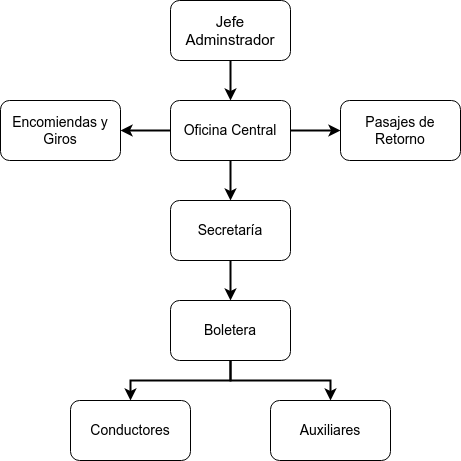
\includegraphics[width=0.55\textwidth]{imagenes/figura1_1.png} % Inserta una imagen
		
		\begin{flushleft}
			\hspace{1.20cm} \textbf{Nota.} Organigrama obtenido en entrevista con el administrador. % Nota al pie para esta figura
		\end{flushleft}
		\vspace{-16pt}
		\label{fig:figura2_1} % Etiqueta para referencia cruzada
	\end{figure}
	
	En la Figura 1, se observa la estructura organizativa del negocio, destacando los diferentes cargos que desempeñan los empleados, que van desde el administrador hasta los auxiliares de apoyo. Dentro del negocio, se encuentran los boleteros y conductores, quienes son responsables de la atención directa a los pasajeros y la operación de los vehículos. Paralelamente, en la oficina central se gestionan las encomiendas, que son recibidas, clasificadas y preparadas para su envío. Cada uno de estos roles desempeña una función esencial para el funcionamiento eficiente y efectivo de la empresa, asegurando que tanto el transporte de pasajeros como la gestión de encomiendas se realicen con éxito y dentro de los estándares de calidad establecidos.
	
	\subsection*{Misión de la empresa}
	
	Proporcionar servicios de transporte y logística de alta calidad, enfocándose en la venta de pasajes y el envío de encomiendas, con el objetivo de satisfacer plenamente las necesidades de nuestros clientes. Nos comprometemos a ofrecer un servicio eficiente, seguro y confiable, contribuyendo al bienestar y comodidad de nuestros usuarios.
	
	\subsection*{Visión de la empresa}
	
	Ser la empresa líder en el sector del transporte y la logística en Bolivia, reconocida por nuestra innovación, eficiencia operativa y excelencia en el servicio al cliente. Aspiramos a expandir nuestra presencia y mejorar continuamente nuestros servicios para mantenernos a la vanguardia de la industria.
	
	\subsection*{Objetivo general de la empresa}
	El objetivo general de Cali Internacional es consolidar y expandir nuestra posición en el mercado del transporte y la logística, mejorando continuamente la calidad de nuestros servicios y adoptando tecnologías avanzadas para optimizar nuestras operaciones y satisfacer las necesidades cambiantes de nuestros clientes.
	
	\subsection*{Objetivos específicos de la empresa}
	
	\begin{itemize}[label=$\bullet$, left=0cm, labelsep = 1.05cm, topsep = 0pt, parsep = 0pt]
		
		\item Mejorar la experiencia del cliente mediante la oferta de servicios más rápidos, seguros y fiables.
		
		\item Capacitar continuamente a nuestro personal para asegurar que estén equipados con las habilidades necesarias para manejar las nuevas tecnologías y brindar un servicio de alta calidad.
		
		\item Implementar prácticas sostenibles en nuestras operaciones, minimizando el impacto ambiental y promoviendo la responsabilidad social corporativa.
		
	\end{itemize}	
	
	\subsection{Antecedentes de proyectos similares}
	
	Para la presente investigación se han considerado los siguientes antecedentes:
	
	\textcite{hurtado2019aplicacion}. ``Aplicación web administrativa para reserva de servicios de transporte y envío de encomiendas para la empresa Romero y Asociados (AMBASEUR) de la ciudad de Ambato''. En este proyecto, se implementó una aplicación web para automatizar los procesos manuales de una empresa, mejorando la gestión de reservas de transporte y envíos de encomiendas. La plataforma permite publicitar las actividades de la empresa y recopilar información precisa sobre los clientes. Desarrollada utilizando la metodología XP, la aplicación facilita la adaptación rápida a cambios y la incorporación de funciones adicionales, como un chat en línea, optimizando así la eficiencia y aumentando la base de clientes.
	
	\textcite{mora2022sistema}. ``Sistema gestión de servicio de viajes para la empresa Nuestra Señora de la Asunción C.I.S.A.'', esta investigación se centra en automatizar los procesos manuales de la empresa Nuestra Señora de la Asunción CISA mediante un sistema informático. En la primera etapa, se diagnosticaron los módulos de viajes, tráfico y ventas, entrevistando a responsables clave y recopilando los requerimientos necesarios. En la segunda etapa, se desarrolló un sistema informático web responsive que procesa automáticamente la información de estos módulos, integrando análisis, diseño y programación orientada a objetos, culminando en un sistema integrado con soporte audiovisual.
	
	\textcite{arevalo2021desarrollo}. ``Desarrollo de una aplicación web para
	agilizar los procesos de la compra y venta de boletos de buses interprovinciales en el terminal de Milagro.'', este proyecto desarrolló un sistema web para la compra y venta de boletos en el terminal terrestre del Cantón Milagro, con el objetivo de agilizar el proceso de boletería sin necesidad de contacto físico en ventanilla. Tras entrevistar a los socios del terminal para identificar los requisitos funcionales y no funcionales, se eligió la metodología ágil SCRUM para la organización y monitoreo constante del proyecto. El sistema se implementó utilizando Python, con Pycharm como IDE, Bootstrap 4 y Adminlte3 como plantillas, y PostgreSQL como base de datos. El resultado fue un sistema que satisface las necesidades del cliente, mejorando significativamente la experiencia de compra de boletos..
	
	\textcite{sosa2019sistema}. ``Sistema informático web para la gestión de pasajes de la empresa de transporte Turismo Transol Barranca S.A.C.'', en la tesis se propone como objetivo principal desarrollar un sistema informático web para la gestión de pasajes en la empresa de transportes Turismo Transol Barranca S.A.C., abarcando tanto la venta como la reserva de boletos. Este sistema busca optimizar el tiempo de procesamiento mediante el uso de tecnología web. La investigación se llevó a cabo con un enfoque descriptivo, un diseño no experimental y un corte transversal, utilizando una población de 42 personas y una muestra de 6 usuarios. Se aplicó la metodología Proceso Unificado de Rational (RUP), empleando el Lenguaje de Modelamiento Unificado (UML) para la construcción de diagramas de casos de uso, facilitando el análisis del software. El sistema fue desarrollado en Java, con MySQL como gestor de datos y MySQL Workbench 6.3 CE para el modelado de la base de datos, entre otras herramientas que ayudaron a cumplir los requisitos de diseño. Los resultados permitieron agilizar los procesos de venta y reserva de pasajes, mejorando el manejo de la información y extendiendo el alcance a los clientes, lo que fortaleció el posicionamiento competitivo de la empresa a nivel regional.
	
	\textcite{vivas2019propuesta}. ``Propuesta de implementación del sistema web de venta de boletos de viaje y gestión de encomiendas para la empresa Transportes Montero S.A.C. Piura; 2018.'', en esta investigación que fue desarrollada por la Escuela Profesional de Ingeniería de Sistemas de la Universidad Católica Los Ángeles de Chimbote, se centró en la mejora de procesos en organizaciones peruanas mediante la implementación de un sistema web para la venta de boletos y gestión de encomiendas en la empresa TRANSPORTES MONTERO S.A.C. en 2018. La investigación, de tipo cuantitativo y descriptivo con diseño no experimental y corte transversal, incluyó una muestra de 14 trabajadores. Los resultados mostraron que el 63 por ciento de los empleados consideraba que la empresa brindaba calidad en procesos y servicios, el 84 por ciento creía que los sistemas web agilizan los procesos, y el 81 por ciento opinaba que dichos sistemas eran eficientes, confirmando así la hipótesis planteada.
	
\section{OBJETO DE ESTUDIO}

	Software de logística y gestión de buses para transporte de pasajeros y envío de encomiendas, el cual va automatizar y mejorar venta de pasajes, así como en la recepción, procesamiento y envío de encomiendas.
	
\section{PLANTEAMIENTO DEL PROBLEMA}

	La empresa de transporte Cali Internacional, se encuentra ante diversos retos importantes en cuanto a administrar sus procesos tanto de venta de pasajes como de envío de paquetería, estas operaciones son llevadas a cabo de forma manual, lo que genera ineficiencias en el funcionamiento, largos tiempos de espera para los clientes y una alta posibilidad de comoter errores. Además de afectar negativamente la experiencia del cliente, estos problemas también restringen las posibilidades de crecimiento y competencia efectiva en un mercado cada vez más digital, la implementación de soluciones tecnológicas integrales se ha convertido en una estrategia clave para optimizar procesos.  
	
	Algunos de los problemas mas frecuentes son:
	
	\begin{itemize}[label=$\bullet$, left=1.25cm, labelsep = 0.75cm, topsep = 0pt, parsep = 0pt]
		\item Largos tiempos de espera en la compra de pasajes y envío de encomiendas debido a la falta de automatización.
		\item Errores en la gestión de reservas y envíos, lo que puede resultar en pérdidas financieras y descontento entre los clientes.
		\item Falta de visibilidad y control sobre la demanda de servicios, lo que limita la capacidad de la empresa para ajustar su oferta y optimizar recursos.
		\item Dificultad para generar reportes y análisis que ayuden en la toma de decisiones estratégicas para la empresa.    
	\end{itemize}
	
	Por lo tanto, se plantea la siguiente interrogante:
	
	?`Cómo mejorar la venta de pasajes y la gestión de envío de encomiendas en la empresa Cali Internacional?
	
\section{JUSTIFICACIÓN}

	La implementación de un software de logística y gestión de buses para transporte de pasajeros y envío de encomiendas representa una respuesta estratégica ante la creciente demanda de soluciones tecnológicas en el sector de transporte y logística. La automatización de estos procesos no solo optimiza las operaciones internas, sino que también reduce significativamente los errores humanos y mejora la eficiencia. En vista de ello la mayoría de organizaciones se ha visto obligada a desarrollar un sistema web de calidad que brinde un mejor servicio a la comunidad, mejorando su imagen corporativa, demostrando que están al día con las nuevas tecnologías \parencite{nunez2005diseno}.
	
	Además, este proyecto aborda la necesidad de ofrecer un servicio más accesible y conveniente para los clientes. En un entorno donde la digitalización se ha vuelto imprescindible, la adopción de un sistema informático para estos servicios es una ventaja competitiva que no se puede ignorar.
	
	La digitalización de estos procesos en una plataforma única no solo agilizará las operaciones al automatizar tareas repetitivas y reducir la necesidad de intervención manual, sino que también mejorará significativamente la precisión y la transparencia de la información. Esta mejora permitirá a la empresa ofrecer un servicio más coherente y eficiente, ya que todos los datos estarán centralizados y accesibles en tiempo real, lo que facilitará una gestión más efectiva de los recursos. Además, la integración de estos procesos en una sola plataforma reducirá costos operativos al eliminar redundancias y optimizar el uso de la infraestructura tecnológica. En última instancia, esto resultará en una mejor experiencia para el cliente, aumentando su satisfacción al recibir un servicio más rápido y confiable, y posicionando a la empresa como líder en innovación y eficiencia dentro de su sector.
	
	Este proyecto se adapta a la necesidad de mantenerse al día con las tendencias tecnológicas actuales. Las empresas están siendo revolucionadas por la transformación digital, y aquellas que no se adapten corren el riesgo de quedarse atrás. Cuando la empresa implementa un software especializado, no solo se adapta a estas tendencias, sino que también está preparada para hacer frente a los desafíos futuros como la necesidad de incorporar nuevas tecnologías y responder a las demandas del mercado en constante cambio.
	
\section{OBJETIVOS}
	\subsection{Objetivo general}
	
		Desarrollar un software de logística y gestión de buses para transporte de pasajeros y envío de encomiendas para la empresa Cali Internacional de la ciudad de La Paz.
		
	\subsection{Objetivos específicos}
	
		\begin{itemize}[label=$\bullet$, left=0cm, labelsep = 1.05cm, topsep = 0pt, parsep = 0pt]
			
			\item Analizar los procesos actuales de venta de pasajes y envío de encomiendas en la empresa Cali Internacional para identificar las áreas de mejora y las necesidades tecnológicas específicas.
			\item Diseñar una interfaz de usuario intuitiva y accesible que permita a los empleados y clientes interactuar con el sistema de manera sencilla, facilitando la usabilidad del software.
			\item Elaborar el diseño de la base de datos a partir del análisis de los requerimientos del sistema, para llevar a la Tercera Forma Normal (3FN) y almacenar los datos.
			\item Diseñar el back-end para gestionar la venta de pasajes y el envío de encomiendas, asegurando la integración eficiente con la base de datos y la correcta ejecución de las operaciones solicitadas por los usuarios a través de la plataforma digital.    
			\item Generar reportes y análisis de datos que facilite la toma de decisiones informadas por parte de la administración de la empresa.
			
		\end{itemize}
		
\section{ALCANCES Y LÍMITES}
	\subsection{Alcances}
		
		El desarrollo de la presente investigación se encuentra dentro de los siguientes alcances:
		
		\begin{itemize}[label=$\bullet$, left=0cm, labelsep = 1.05cm, topsep = 0pt, parsep = 0pt]
			
			\item El proyecto abarcará la creación de una plataforma digital que permita a los usuarios realizar la compra de pasajes y la gestión de envíos de encomiendas de manera eficiente y segura.
			
			\item Se desarrollará un sistema de gestión de usuarios que permitirá a los empleados: iniciar sesión y gestionar las ventas de pasajes y envíos de encomiendas, mientras que los administradores podrán supervisar y manejar las operaciones.
			
			\item Se implementarán módulos que automatizarán tareas repetitivas como la generación de recibos, el seguimiento de envíos y la asignación de asientos en los transportes.
			
			\item El sistema incluirá un módulo de reportes que permitirá a los administradores generar informes detallados sobre las ventas, la ocupación de los transportes, y la gestión de encomiendas.
			
			\item La plataforma será accesible desde diferentes tipos de dispositivos, incluyendo computadoras, tabletas, y smartphones, garantizando una experiencia de usuario consistente y accesible.
			
		\end{itemize}
		
	\subsection{Límites}
	
		Los límites de la investigación son los siguientes:
		
		\begin{itemize}[label=$\bullet$, left=0cm, labelsep = 1.05cm, topsep = 0pt, parsep = 0pt]
			
			\item El sistema estará diseñado inicialmente para cubrir las operaciones de la Empresa Cali Internacional en su sede de la Terminal de Buses en La Paz.
			
			\item La integración se centrará en los sistemas internos existentes de la empresa. %dejando de lado conexiones con plataformas o sistemas externos.
			
			\item El software será compatible con las plataformas y dispositivos especificados. %sin incluir soporte para otros sistemas no contemplados inicialmente.
			
			\item El soporte se limitará a las funcionalidades implementadas, las actualizaciones o desarrollos adicionales quedarán para fases futuras.
			
		\end{itemize}
		
\section{IMPORTANCIA DEL ESTUDIO}

	La importancia del estudio del proyecto radica en la necesidad de modernizar los procesos operativos de empresas de transporte y logística, especialmente en un entorno donde la eficiencia y la rapidez son factores clave para la competitividad. En la actualidad, muchas empresas en este sector aún dependen de sistemas manuales o desactualizados que ralentizan las operaciones, sino que también incrementan el riesgo de errores humanos, afectando directamente la calidad del servicio ofrecido al cliente. Este proyecto, por lo tanto, no solo aborda una necesidad tecnológica, sino que también busca mejorar la experiencia del cliente al ofrecerle un servicio más ágil y fiable.
	
	Desde una perspectiva social, este estudio tiene una importancia significativa al contribuir al avance tecnológico en un sector que afecta directamente a un gran número de personas. Al mejorar la eficiencia y la precisión en la venta de pasajes y el envío de encomiendas, se generan beneficios directos no solo para la empresa, sino también para los usuarios finales, quienes experimentarán un servicio más confiable y accesible. Esto, a su vez, puede fomentar una mayor confianza en los servicios digitales en general, impulsando el uso de la tecnología en otras áreas de la vida diaria.
	
	Finalmente, la importancia de este estudio también reside en su capacidad para servir como modelo para futuras implementaciones tecnológicas en empresas similares. La metodología empleada, así como los desafíos superados durante el desarrollo del software, pueden ofrecer valiosas lecciones para otros proyectos dentro del sector, promoviendo un enfoque más sistemático y eficiente en la adopción de tecnologías de la información en la industria del transporte y la logística.
	
	Introduccion Capítulo 2
	
	Introduccion Capítulo 3
	
	Introduccion Capítulo 4
	
	% Marco teórico
	\chapter{MARCO TEÓRICO} 
	
	\vspace{0pt}
	
	\section{LOGÍSTICA DEL TRANSPORTE DE PASAJEROS}
	\subsection{Logística}
		``Logística es planificar, operar, controlar y detectar oportunidades de mejora del proceso de flujo de materiales (insumos, productos), servicios, información y dinero.  Es la función que normalmente opera como nexo entre las fuentes de aprovisionamiento y suministro y el cliente final o la distribución.  Su objetivo es satisfacer permanentemente la demanda en cuanto a cantidad, oportunidad y calidad al menor costo posible para la empresa.''\parencite{carro2013logistica}
	\subsection{Transporte}
		Según \textcite{koch2001transporte}: ``El concepto de “transporte” hace referencia al traslado de personas y mercancías de un lugar a otro por diversas razones en el menor tiempo posible. En el caso de las personas, destacan los motivos laborales, de estudio o de satisfacción de otras necesidades como el ocio, el acceso a servicios de salud, entre otros; en
		el caso de las mercancías, la necesidad de producción de bienes industriales y de consumo y la posterior comercialización de estos hacen del proceso de transporte un elemento central.'' Por su parte en la \textcite{ley2011transporte}: ``Se denomina transporte al traslado de un lugar a otro de personas y carga.''
		
		
		El transporte es un componente de la logística, que se refiere al conjunto de recursos y estrategias utilizados para organizar un servicio o administrar una empresa. En el ámbito comercial, la logística se relaciona con el envío de productos al lugar adecuado, en el momento correcto y bajo las condiciones necesarias. Por lo tanto, el transporte de mercancías es una parte integral de la logística. El propósito de una empresa es asegurar que la distribución y venta de sus productos se realice de manera eficiente y al menor costo posible. En este contexto, el transporte abarca tanto los vehículos como las infraestructuras asociadas, como camiones, barcos, trenes de carga, carreteras y puertos.
		
		También existen dos tipos de transporte, el público y el privado.
		
		Se habla de transporte público, para hacer referencia a los autobuses, trenes y otras unidades móviles que sirven para la movilización de los ciudadanos de una comunidad y que está solventado y manejado por el Estado vigente. Cabe señalar que en algunos casos, dichos coches pertenecen a empresas privadas que tienen algún tipo de acuerdo con el gobierno y han asumido la responsabilidad de brindar un servicio determinado a la comunidad. Resulta importante señalar que esta clase de transporte no tiene como propósito la generación de ganancias, sino que debe cumplir con un fin social y ser útil para la comunidad. Por ejemplo: “Los transportes públicos están colapsados y requieren de mayores inversiones para
		poder satisfacer las necesidades de la población”.
		
		El transporte privado, en cambio, es el que pertenece a individuos o empresas particulares. En este caso los responsables de la manutención de dichos vehículos son sus dueños, al igual que serán quienes respondan por ellos en caso de
		accidente.
	\subsection{Pasajero}
		En la \textcite{ley_municipal2012transporte} en su artículo 59 se define a los usuarios o pasajeros como ``Las personas naturales o jurídicas que utilizan un vehículo del servicio público o privado de transporte, para trasladarse de un origen a un destino a cambio de una tarifa establecida o remuneración convenida, son considerados usuarios o pasajeros en el marco de la presente Ley Municipal.''
	
	\subsection{Sistema de transporte}
		De acuerdo con \textcite{garcía2016gestión}: ``Un sistema de transporte desde la perspectiva informática es una red interconectada de componentes físicos y digitales que utiliza tecnologías avanzadas de información y comunicación para optimizar el flujo de personas y mercancías. Incluye sistemas de gestión de tráfico, planificación de rutas en tiempo real, control de flotas y plataformas de información al usuario, todos ellos integrados mediante software especializado y bases de datos.''
	% \subsection{Funcionalidad del transporte}
	\section{RESERVA Y VENTA DE PASAJES}
	\subsection{Proceso de reserva y venta de pasajes}
		El proceso de reserva y venta de pasajes es un componente fundamental en la operación de cualquier empresa de transporte de pasajeros. Según \textcite{aparicio2013gestion}, este proceso implica una serie de pasos secuenciales que permiten al cliente asegurar su lugar en un viaje específico. Tradicionalmente, las empresas de transporte han utilizado diversos canales para la reserva y venta, incluyendo puntos de venta físicos, call centers, y más recientemente, plataformas en línea.	
	\subsection{Emisión y gestion de boletos}
		La emisión y gestión de boletos es un proceso crítico que ha evolucionado significativamente con la tecnología. \textcite{agenjo2008transporte} describen dos tipos principales de boletos en el transporte moderno: los electrónicos (e-tickets) y los impresos tradicionales. Independientemente del formato, los boletos deben contener información esencial como datos del pasajero, detalles del viaje, asiento asignado y un método de validación.
		
		El proceso de emisión, según \textcite{garcía2016gestión}, debe ser ágil y estar vinculado directamente con la confirmación del pago. La gestión eficiente de boletos implica un sistema robusto de validación, ya sea en terminales o a bordo de los vehículos, así como la capacidad de reimpresión en caso de pérdida. Además, como señala \textcite{robuste2005logistica}, el seguimiento y registro de los boletos emitidos es importante para el control operativo y financiero de la empresa de transporte.
	\subsection{Cambios y cancelaciones}
		La gestión de cambios y cancelaciones es un aspecto delicado que requiere un equilibrio entre la flexibilidad para los clientes y la protección de los intereses de la empresa. Según \textcite{tejero2015transporte}, las políticas de cambios y cancelaciones deben ser claras, especificando plazos permitidos y cargos aplicables.
		
		El proceso de solicitud de cambios, como describe \textcite{ramírez2015logística}, implica la verificación de disponibilidad para nuevas fechas y el cálculo de diferencias tarifarias. En cuanto a las cancelaciones, el sistema debe determinar el monto del reembolso según la política establecida. La gestión de reembolsos, de acuerdo con \textcite{garcía2016gestión}, debe ser eficiente y transparente, ofreciendo múltiples métodos según las preferencias del cliente.
		
		Un aspecto importante señalado por \textcite{rivera2002ESTUDIODL} es la reasignación de asientos liberados, lo que permite optimizar la ocupación de los vehículos. Además, el registro detallado de cambios y cancelaciones proporciona datos valiosos para el análisis de patrones de comportamiento de los clientes y la mejora continua de los servicios.
		
		En conjunto, estos procesos de reserva, emisión de boletos y gestión de cambios y cancelaciones forman la columna vertebral de la operación de venta de pasajes en una empresa de transporte. Su eficiente implementación y gestión son cruciales para la satisfacción del cliente y el éxito operativo de la empresa.
	\section{LOGÍSTICA DE ENVÍO DE ENCOMIENDAS}
	\subsection{Encomienda}
		La encomienda es el objeto o paquete que se transporta de un punto a otro a través de un servicio de mensajería o transporte. Según \textcite{stock2000strategic}, ``una encomienda representa una unidad logística que debe ser gestionada y tratada como tal, garantizando su integridad desde el origen hasta el destino final''. En el contexto del transporte de encomiendas, es fundamental contar con un sistema que permita la correcta identificación, seguimiento y gestión de cada paquete.
		
		\textcite{garcía2016gestión} destaca que el concepto de encomienda ha evolucionado con el tiempo, especialmente con el auge del comercio electrónico. Actualmente, las empresas de transporte deben estar preparadas para manejar una amplia gama de artículos, desde documentos hasta productos perecederos, cada uno con sus propios requisitos de manipulación y transporte. Esta diversidad exige sistemas flexibles y adaptables que puedan responder a las necesidades cambiantes de los clientes y del mercado.
	\subsection{Proceso de recepción}
		El proceso de recepción es la primera etapa en la gestión de encomiendas, donde se verifica la información proporcionada por el remitente, se inspecciona el paquete y se registran los detalles necesarios para su envío. De acuerdo con \textcite{garcía2016gestión}, este proceso implica la verificación inicial del paquete, el registro de información relevante y la asignación de un identificador único. \textcite{escudero2019logistica} enfatiza la importancia de este paso para garantizar la trazabilidad y el manejo adecuado de la encomienda durante todo su trayecto.
		
		Con el avance de las tecnologías, muchas empresas han implementado sistemas que automatizan el proceso de recepción, permitiendo la digitalización de la información desde el inicio del proceso logístico. Esto facilita un flujo continuo de datos entre las distintas etapas del envío, reduciendo errores humanos y optimizando los tiempos de procesamiento.
	\subsection{Clasificación de encomiendas}
		La clasificación de encomiendas es un paso fundamental para optimizar el proceso de envío. Según \textcite{i2001manual}, las encomiendas se pueden clasificar según diversos criterios, como tamaño, peso, destino, urgencia o tipo de contenido. \textcite{tejero2015transporte} señala que una clasificación eficiente permite una mejor planificación de rutas y utilización de los espacios de carga.
		
		\textcite{escudero2019logistica} agrega que la clasificación también juega un papel crucial en la priorización de los envíos y la asignación de recursos. Por ejemplo, las encomiendas urgentes o perecederas pueden requerir un tratamiento especial y rutas más directas. Además, una clasificación adecuada facilita el cumplimiento de regulaciones específicas, como las relacionadas con el transporte de mercancías peligrosas o artículos restringidos.
	\subsection{Embalaje y etiquetado}
		El embalaje y etiquetado son procesos críticos para garantizar la integridad y correcta identificación de las encomiendas. \textcite{ramírez2015logística} destaca que el embalaje debe proporcionar protección adecuada según la naturaleza del contenido y las condiciones del transporte. Esto puede incluir el uso de materiales de amortiguación, envoltorios impermeables o contenedores especializados para artículos frágiles o sensibles a la temperatura.
		
		El etiquetado, por su parte, es igualmente importante, ya que proporciona la información necesaria para la correcta identificación del paquete. Esta información incluye los datos del remitente y del destinatario, instrucciones especiales de manejo y, en muchos casos, códigos de seguimiento que permiten rastrear el paquete en tiempo real. \textcite{ballou2004logistica} menciona que un etiquetado claro y preciso es esencial para evitar errores en la clasificación y garantizar que el paquete llegue a su destino de manera eficiente. Las tecnologías modernas, como los códigos QR, también han facilitado este proceso, permitiendo una gestión más ágil de los envíos.
	\subsection{Entrega al destinatario}
		La entrega al destinatario es la fase final en la logística de encomiendas, y su éxito depende en gran medida de la eficiencia de los pasos previos. Según \textcite{garcía2016gestión}, este proceso implica la verificación de la identidad del destinatario, la obtención de una firma de recepción y la resolución de cualquier incidencia que pueda surgir. \textcite{tejero2015transporte} resalta la importancia de la puntualidad y la integridad de la entrega como factores clave en la satisfacción del cliente y la reputación de la empresa de transporte.
		
		Sin embargo, la entrega puede enfrentarse a diversos retos, como la ausencia del destinatario en el momento de la entrega o dificultades de acceso en ciertas áreas geográficas. Para contrarrestar estos problemas, empresas líderes en logística han implementado políticas de entrega flexible, que permiten a los clientes seleccionar franjas horarias de entrega, puntos de recogida o reprogramar la entrega.
	\section{GESTIÓN DE BUSES}
	\subsection{Asignación de rutas}
		La asignación de rutas es uno de los procesos clave en la gestión de transporte de pasajeros, ya que su correcta planificación puede mejorar significativamente la eficiencia operativa y la satisfacción del cliente. Según \textcite{molinero2005transporte}, este proceso implica la determinación de los recorridos óptimos que deben seguir los vehículos para cubrir la demanda de pasajeros de manera eficiente. Los autores señalan que una asignación de rutas efectiva debe considerar factores como la densidad poblacional, los patrones de viaje de los usuarios, la infraestructura vial disponible y las restricciones operativas de la empresa.
		
		También \textcite{ballou2004logistica} destaca que la planificación de rutas tiene como objetivo maximizar la eficiencia operativa mediante la reducción de distancias y tiempos muertos. Ballou resalta que una asignación óptima de rutas no solo mejora la utilización de los vehículos, sino que también contribuye a una mejor satisfacción del cliente, al reducir los tiempos de entrega y los costos asociados.
	\subsection{Programación y asignación de conductores}
		La programación y asignación de conductores es un componente esencial en la gestión de buses, que busca optimizar el uso del recurso humano y garantizar la operación eficiente de los servicios. Según \textcite{mauttone2002diseno}, este proceso implica la optimización de recursos humanos para garantizar la cobertura eficiente de las rutas y horarios establecidos. \textcite{ibarra2012synchronization} enfatizan la importancia de sincronizar los horarios de los conductores con los tiempos de llegada y salida de los vehículos, lo que no solo mejora la puntualidad del servicio, sino que también reduce los tiempos de espera para los pasajeros. Esta sincronización debe tener en cuenta factores como los períodos de descanso obligatorios, los cambios de turno y las variaciones en la demanda de pasajeros a lo largo del día.
		
		Por otro lado, \textcite{molinero2005transporte} añaden que la programación debe considerar no solo la eficiencia operativa, sino también el bienestar de los conductores, incluyendo aspectos como la fatiga, las preferencias personales y el equilibrio entre trabajo y vida personal. Esto subraya la necesidad de un enfoque holístico que balancee las necesidades operativas con las consideraciones humanas en la gestión del personal de transporte público.	
	
	\section{MARCO LEGAL Y NORMATIVO}
	\subsection{Autoridad de regulación y fiscalización de telecomunicaciones y transportes}
	La Autoridad de Regulación y Fiscalización de Telecomunicaciones y Transportes
	(ATT), es una institución pública, técnica y operativa, con personalidad jurídica y patrimonio propio, independencia administrativa, financiera, legal y técnica, transitoriamente dependiente del Ministerio de Obras Públicas, Servicios y Vivienda, de acuerdo a la Ley 164.
	
	La ATT, tiene como objetivo regular las actividades que realizan las personas
	naturales y jurídicas, privadas, comunitarias, públicas, mixtas y cooperativas en los sectores de telecomunicaciones, transportes, tics y servicios postales, asegurando que se garantice los intereses y derechos de los consumidores y usuarios, los intereses del país y el desarrollo del sector, promoviendo la economía plural e inclusiva prevista en CPE, y brindando posibilidades para que más habitantes puedan acceder a los servicios \parencite{institucion2017memoria}.
	\subsection{Ley general del transporte}
	"Ley Nro. 165 de transporte, El Sistema de Transporte Integral - STI, en todo el 	Estado Plurinacional de Bolivia, se rige por la Constitución Política del Estado, los Tratados, Convenios e Instrumentos Internacionales, la Ley Marco de Autonomías y Descentralización, la presente Ley, normas sectoriales y otras normas específicas del ordenamiento jurídico del Estado Plurinacional.” \parencite{ley2011transporte}
	
	Sus principios son:
	
	\textbf{Accesibilidad.} Todas las usuarias y usuarios podrán acceder al Sistema de
	Transporte Integral - STI, por el medio y modalidad que escojan, los mismos que
	deben contar con facilidades de acceso y estar en condiciones de equidad, calidad y seguridad.
	
	\textbf{Calidad.} El Sistema de Transporte Integral - STI, debe proveer un servicio en
	conformidad a los requisitos y estándares que garanticen un nivel de servicio
	adecuado de bienestar, eficiencia y eficacia, de acuerdo a la contraprestación
	autorizada.
	
	\textbf{Continuidad.} El Sistema de Transporte Integral - STI, debe funcionar de manera
	permanente, regular y continua.
	
	\textbf{Eficacia.} El servicio de transporte debe cumplir el propósito para el cual fue convenido.
	
	\textbf{Eficiencia.} El Sistema de Transporte Integral - STI, debe prestar servicios en condiciones que garanticen el menor costo operacional y tiempo posible, contemplando un nivel de equidad, calidad y seguridad.
	
	\textbf{Participación y control social.} Se garantizará y facilitará la participación y control social sobre la gestión pública por parte de la sociedad civil organizada.
	
	\textbf{Seguridad.} El Sistema de Transporte Integral - STI, debe prestar servicios en condiciones que garanticen la integridad de personas y carga durante el traslado del lugar de origen al lugar de destino.
	
	\textbf{Sostenibilidad.} El sistema de transporte debe prestar servicios que garanticen el menor impacto sobre la salud y el medio ambiente local y global. En el corto, mediano y largo plazo, sin comprometer el desarrollo de futuras generaciones.
	
	\textbf{Transparencia.} Se garantiza la transparencia en el Sistema de Transporte Integral - STI.
	
	\textbf{Universalidad.} Todas las usuarias y usuarios sin distinción alguna, tienen el derecho de utilizar el Sistema de Transporte Integral - STI, para su libre movilidad.
	
	\subsection{Reglamento regulatorio de transporte terrestre de pasajeros y carga}
	
	Resolución Ministerial N° 266 del 14 de agosto de 2017, emitida por el Ministerio de Obras Públicas, Servicios y Vivienda.
	
	\textbf{ARTÍCULO 1 (OBJETO.-)} Reglamentar los aspectos regulatorios del servicio de
	transporte en la modalidad terrestre de pasajeros y carga en aplicación a la Ley N° 165 General de Transporte.
	
	SECCIÓN III: DE LA INFORMACIÓN AL USUARIO Y LAS CONDICIONES	PARA EL VIAJE
	\textbf{ARTÍCULO 14. (INFORMACIÓN AL USUARIO).}
	
	\begin{enumerate}[label=\Roman*., nosep] % Enumeración principal en números romanos
		\item El operador, previamente a la compra del pasaje, debe informar al usuario, de forma clara, precisa y oportuna, sobre lo siguiente:
		\begin{enumerate}[label=\alph*), nosep] % Subítems con letras minúsculas
			\item Destinos, itinerario, rutas, tiempo de viaje, hora de salida y hora estimada de arribo del vehículo al lugar de destino.
			\item Capacidad del vehículo y asientos disponibles de acuerdo a numeración.
			\item Tarifas aprobadas por la Autoridad Regulatoria de acuerdo a las características del servicio de transporte terrestre interdepartamental.
			\item Peso, volumen y cantidad permitidos para el transporte de equipaje facturado y de mano, restricciones del equipaje considerado peligroso y/o nocivo a la salud.
			\item Condiciones del transporte requisitos y documentación necesaria para el viaje al país de destino; condiciones de reembolso en caso que el usuario desista del viaje; entre otros.
		\end{enumerate}
		
		\item El operador tiene la obligación de informar al pasajero antes del inicio y durante el viaje lo siguiente:
		\begin{enumerate}[label=\alph*), nosep]
			\item Características del servicio: destino, fecha, hora del viaje, número y categoría del bus y número de carril.
			\item Derechos y obligaciones de los usuarios.
			\item  Demoras y/o cancelaciones, nueva hora de salida u otros aspectos relacionados al viaje.
			\item Rutas alternativas o desvíos y demoras del viaje por caso fortuito o fuerza mayor durante el viaje.
		\end{enumerate}
	\end{enumerate}
	
	\textbf{ARTÍCULO 15. (ACREDITACIÓN DE INFORMACIÓN PROPORCIONADA AL USUARIO).}
	
	El operador deberá aplicar diferentes mecanismos para brindar información confiable al usuario al momento de la compra del boleto, antes y durante la ejecución del servicio, y al momento de la entrega de carga y/o encomiendas, debiendo cumplir con esta obligación y acreditar tal situación.
	
	\textbf{ARTÍCULO 16. (MECANISMOS DE INFORMACIÓN).}
	
	En los monitores internos del vehículo del operador deben difundir material audiovisual, que informe y dé a conocer a los usuarios sus derechos, obligaciones y prohibiciones.
	
	\textbf{SECCIÓN IV: DEMORA, INTERRUPCIÓN Y/O CANCELACIÓN DEL VIAJE}
	
	\textbf{ARTÍCULO 23. (ATENCIONES AL PASAJERO POR CAUSAS ATRIBUIBLES AL OPERADOR).}
	
	\begin{enumerate}[label=\Roman*.,
		nosep, % Elimina espacio arriba y abajo de la lista
		itemsep=0pt, % Elimina espacio entre los ítems
		parsep=0pt % Elimina espacio entre párrafos dentro de los ítems
		]
		\item En casos de cancelaciones, interrupciones, demoras, duplicidad de boletos o ante cualquier otro evento que sea imputable al operador, éste deberá:
		\begin{enumerate}[label=\alph*),
			nosep, % Elimina espacio entre subítems y la lista
			itemsep=0pt, % Elimina espacio entre los subítems
			parsep=0pt % Elimina espacio entre párrafos dentro de los subítems
			]
			\item Demoras: si la demora fuera mayor a los 15 minutos, informar a los pasajeros la causa y la nueva hora de salida del bus.
			
			Si la demora fuera mayor a una (1) hora, deberán poner a disposición de los pasajeros otro bus de la misma categoría o acordar el transporte de éstos con otro operador.
			
			\item Cancelación: si el viaje es cancelado, deberá embarcar al pasajero en el siguiente bus disponible o de otro operador de idéntica categoría lo más rápidamente posible o en una fecha posterior que convenga al pasajero.
			
			\item Interrupción del viaje: si el viaje es interrumpido después de iniciado por fallas mecánicas y/o accidentes y no pueda continuar el recorrido, el operador se comunicará con su Centro de Contingencias e informará a los pasajeros las medidas a adoptar para auxiliarlos y el tiempo estimado en que llegará el auxilio para continuar el viaje, a fin de que el pasajero tome una determinación: esperar el bus de auxilio o tomar otro medio de transporte para llegar a destino.
			
			\item Duplicación de asientos: ante la venta de dos o más boletos para un solo espacio, deberá asignar al pasajero otro espacio en el bus o embarcarlo en otro bus de igual categoría. Solo a solicitud del usuario deberá rembolsar el 100 por ciento del valor del pasaje.
			
			\item Anticipación del viaje: en caso que el operador anticipe el viaje sin avisar al pasajero, deberá proporcionarle un espacio en el siguiente viaje que le resulte conveniente a su destino final. En estos casos, el pasajero no pagará ningún excedente si el nuevo espacio correspondiera a una tarifa superior. 
		\end{enumerate}
		
		\item En todos los casos, el operador está terminantemente prohibido de recurrir directamente a la devolución; deberá agotar todas las posibilidades para cumplir con el contrato; optará por la devolución únicamente si el pasajero lo requiere.
		
		\textbf{ARTÍCULO 56.- (PROHIBICIONES DEL CONDUCTOR)}
		
		Queda terminantemente prohibido a los conductores de las unidades de servicio de transporte automotor público terrestre en corresponsabilidad con el operador, lo siguiente:
		
		\begin{enumerate}[label=\alph*),
			nosep,
			itemsep=0pt,
			parsep=0pt
			]
			\item Presentarse al trabajo con síntomas de haber ingerido bebidas alcohólicas, o bajo la influencia de sustancias psicotrópicas o ingerirlas en horas de trabajo.			
			\item Transportar pasajeros en los pasillos, buzones y cabina del bus.
			\item Realizar paradas no programadas o desviar el vehículo de su recorrido oficial, a menos que fuera instrucción de las autoridades correspondientes.
			\item Abandonar el vehículo en plena carretera.			
			\item Efectuar paradas no autorizadas cuya duración exceda los 20 minutos.
			\item Agredir físicamente o psicológicamente a los usuarios, personal de la Autoridad Competente, Policía Boliviana u operador del servicio de Terminal Terrestre.			
			\item Usar radios o parlantes con alto volumen de sonido.
			
		\end{enumerate}
		
	\end{enumerate}
		
	\section{INGENIERÍA DE SOFTWARE}
		La Ingeniería de Software es una disciplina dentro de la informática encargada de la aplicación de un enfoque sistemático y metodológico al desarrollo, operación y mantenimiento de sistemas de software de alta calidad. Este campo surgió en respuesta a la creciente complejidad de los sistemas informáticos y a la necesidad de garantizar que los programas y aplicaciones sean confiables, eficientes y ajustados a los requisitos del cliente.
		
		Según \textcite{sommerville2011introduccion}, la ingeniería de software implica la aplicación de principios científicos y de ingeniería en el diseño, desarrollo, prueba y mantenimiento de software. Este enfoque abarca desde el análisis de requisitos, la creación de modelos, la implementación del software, hasta la prueba y verificación del mismo. La clave de la ingeniería de software radica en estructurar cada etapa del proceso de desarrollo de manera que permita crear sistemas que sean fácilmente mantenibles y adaptables a los cambios.
		
		Además, \textcite{pressman2010ingenieria} enfatiza que la ingeniería de software no solo se ocupa del código, sino que integra el manejo de proyectos, la gestión de riesgos y la implementación de técnicas para la verificación de la calidad del producto. Esta disciplina ayuda a gestionar el ciclo de vida completo del software, desde el diseño hasta el mantenimiento, lo cual es esencial en proyectos complejos que requieren altos estándares de calidad y funcionalidad.
		
	\section{MODELO EN CASCADA}
	\subsection{Requerimientos del software}
	\subsection{Diseño del programa}
	\subsection{Codificación}
	\subsection{Construcción y pruebas}
	\subsection{Implantación}
	\section{MODELO ENTIDAD - RELACIÓN}
	\section{BASE DE DATOS}
	\section{HERRAMIENTAS DE DESARROLLO}
	\section{PRUEBAS}
	\section{MODELO DE CALIDAD BOEHM}
		
	
	

	
	
	%\vspace{0.3cm} % Agregar 1 cm de espacio entre el párrafo y la figura
	
	%	\begin{figure}[h] % 'H' del paquete 'float' para mantener posición	
		%		\caption[Descripción corta]
		%		{\newline Resultados del informe PISA 2022.} % Leyenda en la parte superior
		%		\centering
		%		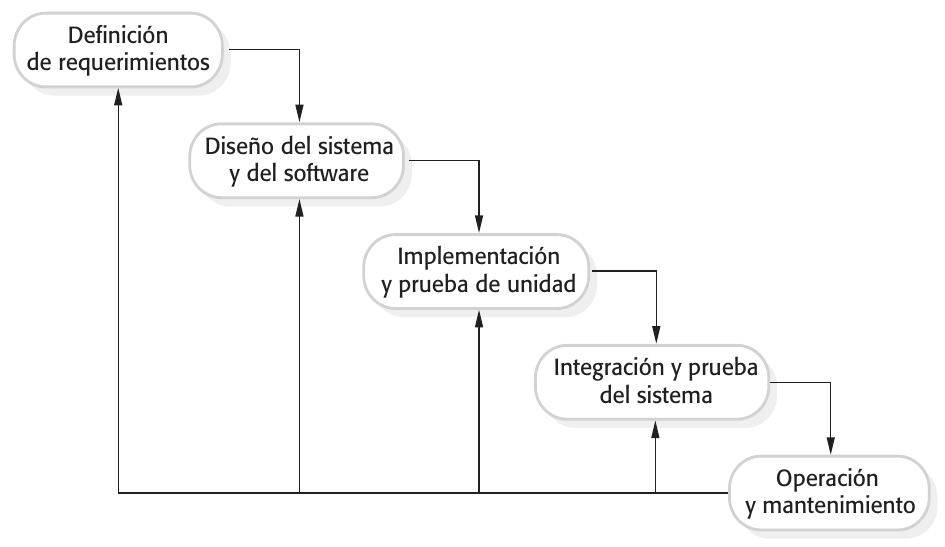
\includegraphics[width=0.95\textwidth]{imagenes/figura2_1.png} % Inserta una imagen
		%		
		%		\begin{flushleft}
			%			\hspace{1.20cm} \textit{Nota.} al pie asociada con esta figura, explicando detalles adicionales. % Nota al pie para esta figura
			%		\end{flushleft}
		%		\vspace{-16pt}
		%		\label{fig:figura2_1} % Etiqueta para referencia cruzada
		%	\end{figure}



	% Marco aplicativo
	\chapter{MARCO APLICATIVO}
\section{ANÁLISIS Y DEFINICIÓN DE REQUERIMIENTOS}
	En la primera etapa del desarrollo del software, se realiza el Análisis y definición de requerimientos, una fase esencial donde se identifican y documentan las necesidades y expectativas del cliente mediante la ingeniería de requerimientos. Esta etapa es importante para asegurar que el desarrollo posterior esté alineado con las metas del proyecto y que el sistema cumpla efectivamente con las expectativas planteadas, evitando problemas en fases avanzadas del desarrollo.
	
	\subsection{Levantamiento de requerimientos}
	Para la realización del levantamiento de requerimientos se realizó un cronograma de reuniones que se observa en la tabla \ref*{tab:tabla3_1}.
	\vspace{-1pt}  % O el valor que necesites para ajustar
	% Nota personalizada fuera de `\caption*{}`
	% \textbf{Nota}: Esta es la nota de la tabla, explicando datos relevantes.
	
	\begin{longtable}{>{\centering\arraybackslash}m{3cm} >{\centering\arraybackslash}m{5cm}}
		\caption[Cronograma de Entrevistas]{\newline Cronograma de reuniones} \label{tab:tabla3_1}\\
		\toprule
		\textbf{Reunión} & \textbf{Fecha}\\
		\midrule
		\endfirsthead
		
		\toprule
		\textbf{Reunión} & \textbf{Fecha}\\
		\midrule
		\endhead
		
		%\midrule
		%\multicolumn{3}{r}{\textit{Continúa en la siguiente página}} \\
		%\midrule
		%\endfoot
		
		\bottomrule
		\endlastfoot
		
		% Aquí se colocan las filas de la tabla, por ejemplo:
		1 & 9/8/2024 \\
		2 & 30/8/2024 \\
		3 & 27/9/2024 \\
		4 & 8/11/2024 \\
		5 & 6/12/2024 \\
		
	\end{longtable}
	\vspace{-12pt}  % O el valor que necesites para ajustar
	% Nota personalizada fuera de `\caption*{}`
	% \textbf{Nota}: Esta es la nota de la tabla, explicando datos relevantes.
	Las entrevistas fueron programadas en base al cronograma detallado en la tabla \ref{tab:tabla3_1}, logrando reuniones efectivas tanto con el administrador y con el personal de atención al cliente. A continuación, se detallan las consultas realizadas en estas sesiones.
		
	\textbf{Entrevista al Administrador}
	
	Información del Entrevistado
	\begin{itemize}[label=$-$, left=0cm, labelsep = 0.9cm, topsep = 0pt, parsep = 0pt]
		\item Cargo: Administrador General
		\item Fecha: 9/8/2024
		\item Lugar: Empresa de Transportes Cali Internacional
		\item Duración estimada: 60 minutos
	\end{itemize}
	
	Preguntas:
	
	\begin{enumerate}[left=0.1cm, labelsep = 0.9cm, topsep = 0pt, parsep = 0pt]
		\item ¿Cuáles son los principales problemas o dificultades que enfrenta la empresa con el manejo actual?
		\item ¿Qué procesos considera que son los más críticos y necesitan mayor atención?
		\item ¿Cómo se gestiona actualmente el control de buses y encomiendas en la empresa?
		\item ¿Cuántos buses tiene actualmente la empresa en operación?
		\item ¿Cuántas rutas manejan y cuáles son sus principales destinos?
		\item ¿Qué problemas son los más frecuentes en el servicio de encomiendas?
		\item ¿Qué volumen promedio de encomiendas manejan diariamente?
		\item ¿Qué funcionalidades específicas necesita que tenga el módulo de gestión de buses para optimizar las operaciones?
		\item ¿Cómo se realiza actualmente la asignación de conductores a las unidades?
		\item ¿Cuántos empleados necesitarán acceso al sistema?
		\item ¿Qué roles o niveles de acceso considera necesarios para el personal?
		\item ¿Qué tipos de reportes son esenciales para la toma de decisiones?
		\item ¿Cómo le gustaría que se maneje el sistema de reservas y venta de pasajes?
		\item ¿Qué sistema de tarifas manejan y cómo les gustaría que se implemente en el software?
		\item ¿Qué tipo de reportes financieros necesita generar periódicamente?
		\item ¿En qué plazo espera que el sistema esté completamente operativo?
	\end{enumerate}
	
	\textbf{Entrevista al Personal de atención al cliente}
		
	Información del Entrevistado
	\begin{itemize}[label=$-$, left=0cm, labelsep = 0.9cm, topsep = 0pt, parsep = 0pt]
		\item Vendedor de pasajes y recepcionista de encomiendas
		\item Fecha: 9/8/2024
		\item Lugar: Empresa de Transportes Cali Internacional
		\item Duración estimada: 60 minutos
	\end{itemize}
	
	Preguntas:
	
	\begin{enumerate}[left=0.1cm, labelsep = 0.9cm, topsep = 0pt, parsep = 0pt]
		\item ¿Cuál es el proceso actual que sigue para vender un boleto de viaje?
		\item ¿Qué información del cliente es obligatoria registrar al momento de la venta?
		\item ¿Cómo maneja las reservaciones de asientos?
		\item ¿Qué problemas son los más frecuentes durante el proceso de venta de boletos?
		\item ¿Cómo gestiona actualmente los diferentes tipos de tarifas?
		\item ¿Cuál es el procedimiento actual para registrar una encomienda?
		\item ¿Qué información necesita registrar sobre las encomiendas?
		\item ¿Cómo realiza el seguimiento de una encomienda cuando un cliente lo solicita?
		\item ¿Qué problemas son los más comunes en el servicio de encomiendas?
		\item ¿Cómo maneja las quejas por pérdida o retraso de encomiendas?
		\item ¿Cuáles son las preguntas más frecuentes de los clientes?
		\item ¿Qué información necesita tener a mano para responder rápidamente a las consultas de los clientes?
		\item ¿Cómo gestiona los cambios o cancelaciones de pasajes?
		\item ¿Cómo realiza el cierre de caja de sus ventas?
		\item ¿Qué tipo de reportes necesita generar durante su turno?
		\item ¿Cómo verifica la disponibilidad de asientos en los buses?
		\item ¿Qué reportes le facilitarían su trabajo diario?
		\item ¿Qué proceso sigue cuando un cliente pierde su boleto?
		\item ¿Qué experiencia tiene en el uso de sistemas informáticos?
		\item ¿Qué aspectos considera importantes incluir en la capacitación del nuevo sistema?
		\item ¿Qué información proporciona a los clientes sobre el viaje?
	\end{enumerate}
	
	Como parte complementaria al proceso de entrevistas, se realizó también la \textbf{técnica de observación directa} de las operaciones diarias en la empresa de transportes durante la semana del 12 al 16 de agosto de 2024. Esta técnica permitió identificar aspectos que no fueron mencionados durante las entrevistas y validar la información proporcionada por el personal.
	
	Durante la observación se identificaron los siguientes aspectos:
	
	\begin{enumerate}[left=0.1cm, labelsep = 0.9cm, topsep = 0pt, parsep = 0pt]
		\item Procesos que requieren optimización:
		\begin{itemize}[label=$-$, left=0cm, labelsep = 0.9cm, topsep = 0pt, parsep = 0pt]
			\item Verificación de disponibilidad de asientos
			\item Registro de encomiendas
			\item Control de embarque de pasajeros
			\item Gestión de caja y turnos
		\end{itemize}		
		\item Puntos críticos identificados:
		\begin{itemize}[label=$-$, left=0cm, labelsep = 0.9cm, topsep = 0pt, parsep = 0pt]
			\item Tiempos de espera prolongados en horas pico
			\item Proceso manual propenso a errores
			\item Falta de información en tiempo real
		\end{itemize}
		\item Oportunidades de mejora:
		\begin{itemize}[label=$-$, left=0cm, labelsep = 0.9cm, topsep = 0pt, parsep = 0pt]
			\item Automatización del proceso de venta
			\item Gestión digital de asientos
			\item Control automatizado de embarque
		\end{itemize}
	\end{enumerate}
	
	La observación directa permitió complementar la información obtenida en las entrevistas y proporcionó una visión más clara de los procesos actuales y las necesidades reales de automatización.

	\subsection{Análisis de requerimientos}
	Durante la fase de Análisis de requerimientos del proyecto, se realizó un proceso integro para definir y estructurar los casos de uso que abarcarán las funcionalidades esenciales del sistema, esta etapa se centró en organizar las interacciones clave que los usuarios tendrán con el sistema, permitiendo establecer una visión clara de cómo deben funcionar los distintos módulos.
	
	En esta fase se realizó la organización y documentación de los casos de uso, lo que facilitó el establecimiento de una visión clara de las funcionalidades a desarrollar, se logró crear una especificación detallada de cada caso de uso, incluyendo actores, flujos principales, flujos alternativos y condiciones específicas de ejecución. Este nivel de detalle proporciona una guía clara para las fases subsecuentes del proyecto, también permite establecer un entendimiento común con los interesados sobre cómo el sistema debe comportarse ante las diferentes interacciones de los usuarios.\\
	\textbf{Diagrama de casos de uso}
		
	De acuerdo al análisis de requerimientos en la figura \ref{fig:caso_uso}, se presenta el Diagrama de casos de uso identificados para el sistema.
	
	\begin{figure}[!h] % 'H' del paquete 'float' para mantener posición	
		\caption[Diagrama de Casos de Uso]
		{\newline Diagrama de Casos de Uso} % Leyenda en la parte superior
		\vspace{0.3cm}
		\centering
		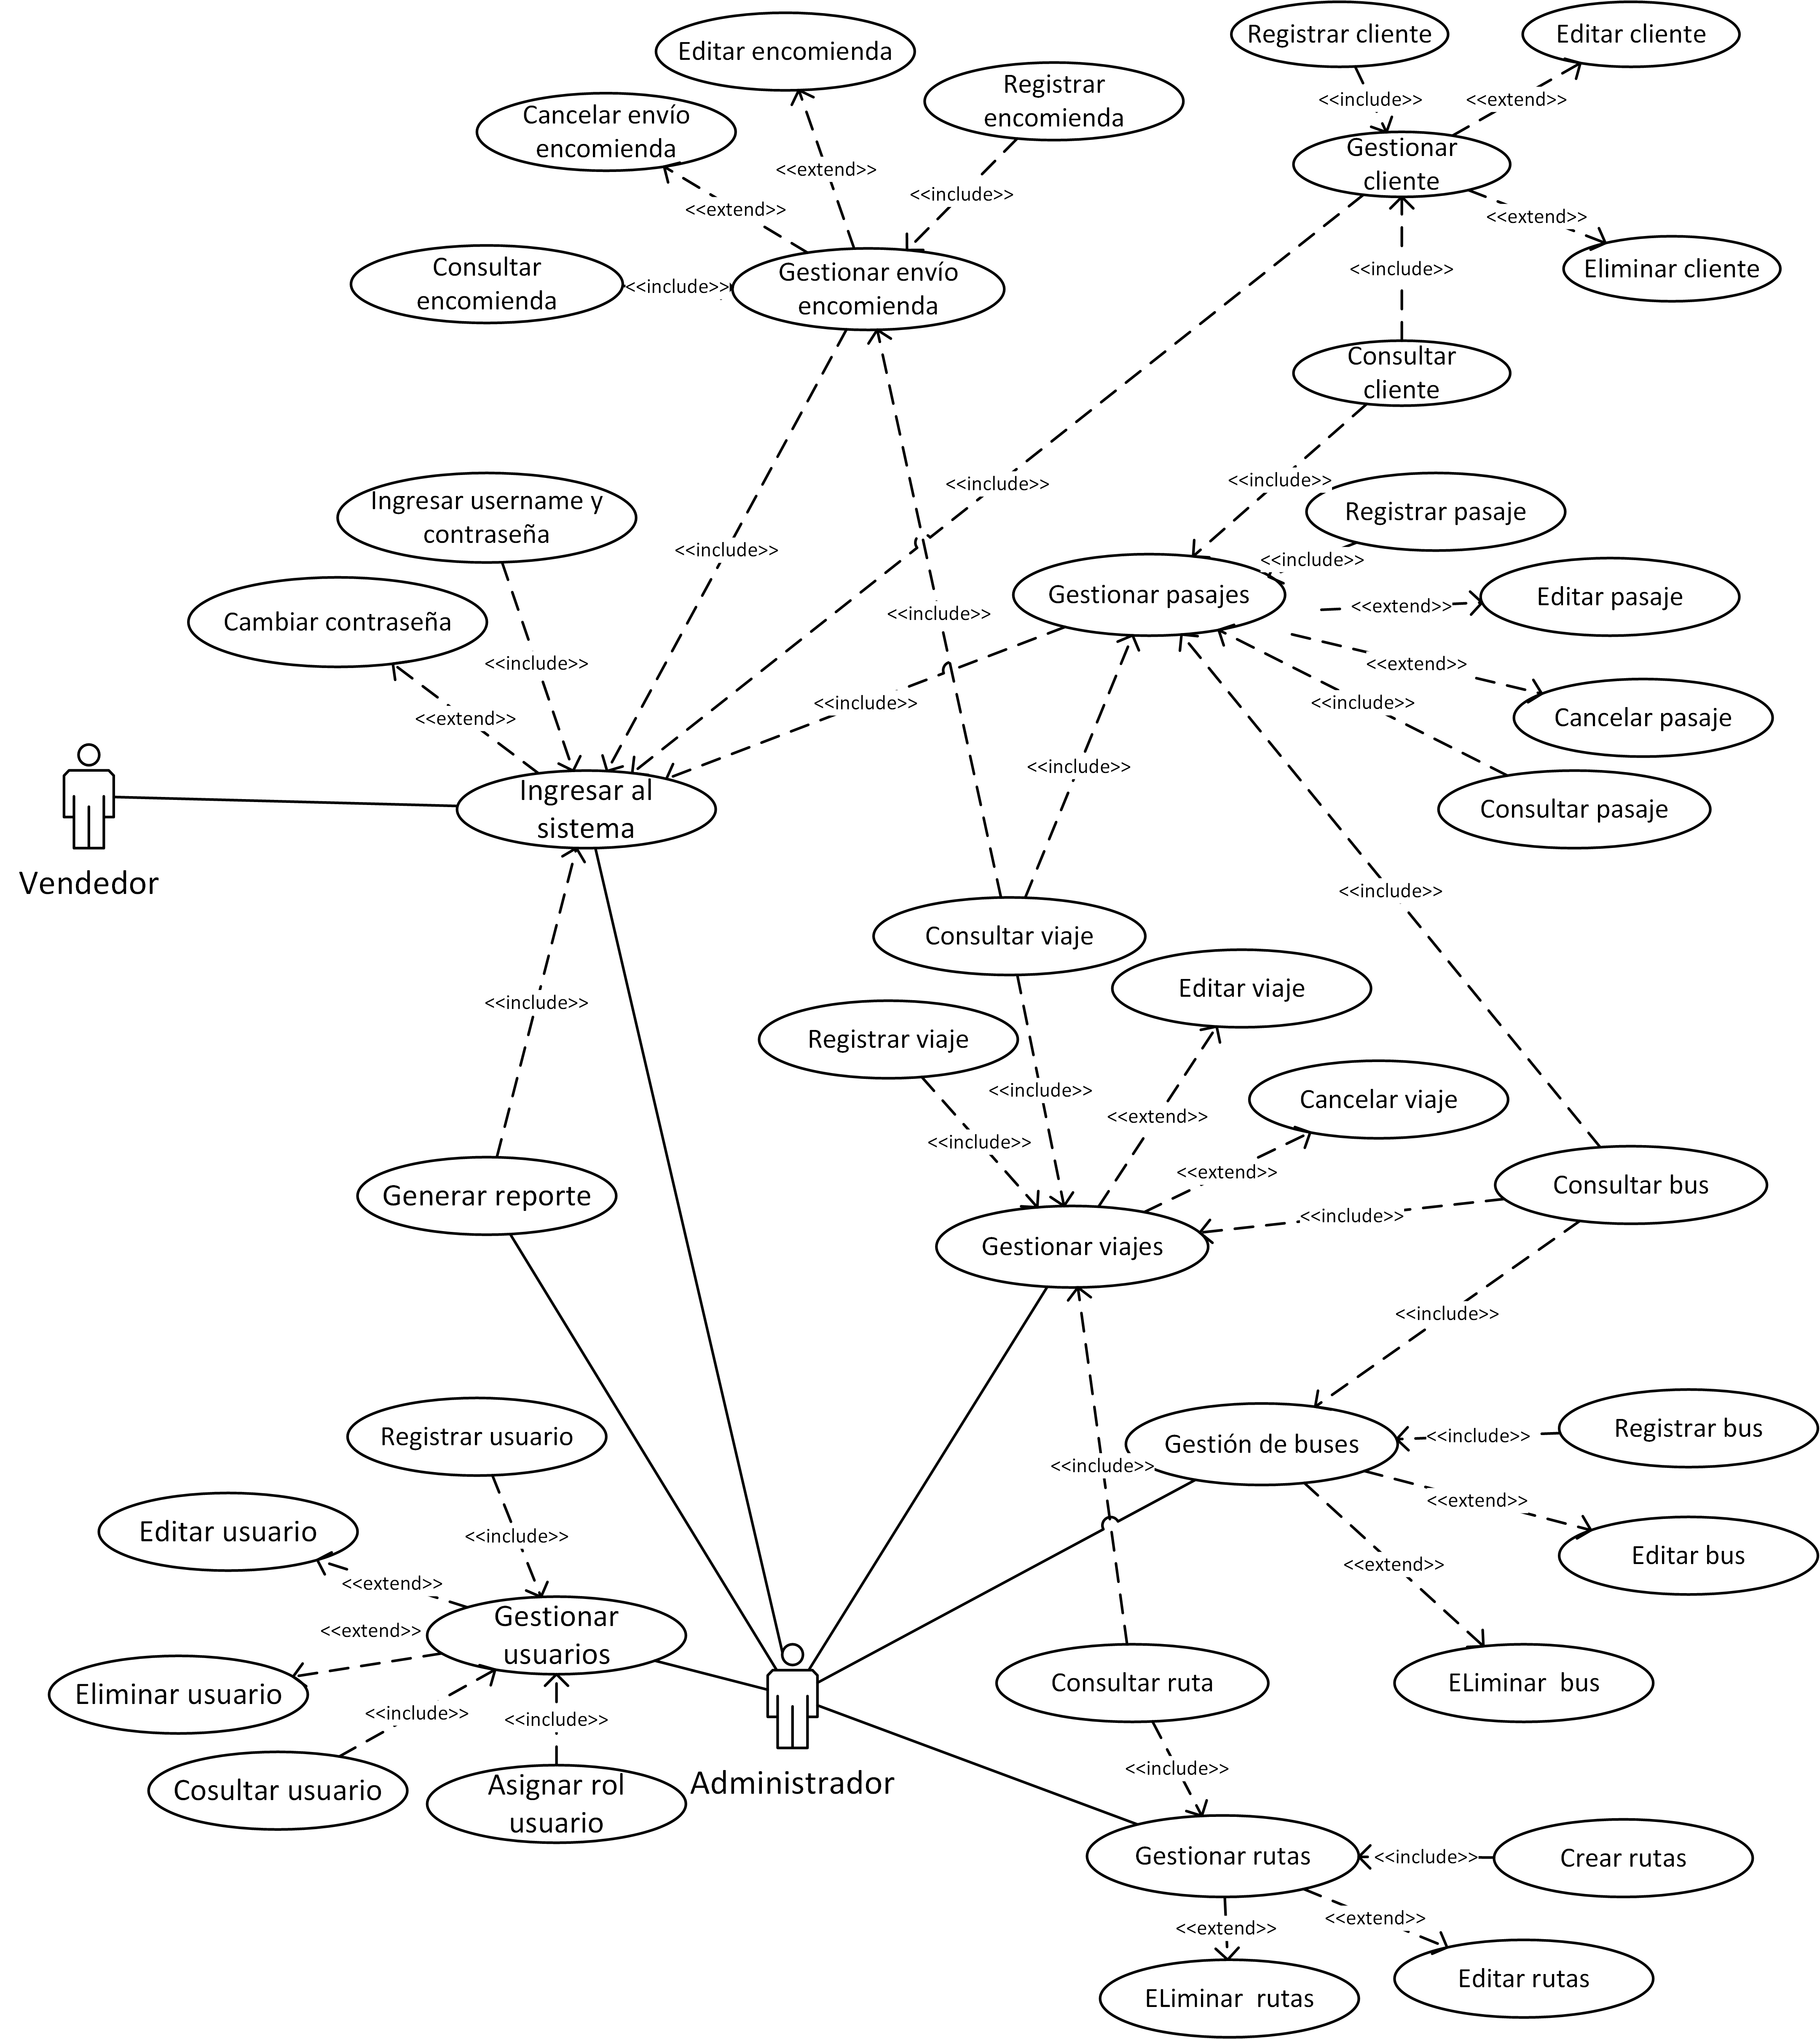
\includegraphics[width=1\textwidth]{imagenes/cap_3/casos_de_uso.png} % Inserta una imagen
		\vspace{0.3cm}
		%\caption*{\textup{\textbf{Nota}: Obtenido de https://evaluacionred-g3-2019.fandom.com/}}
		\vspace{-0.8cm}
		\label{fig:caso_uso} % Etiqueta para referencia cruzada
	\end{figure}
	
	\noindent \textbf{Especificaciones de casos de uso}
	
	El presente apartado desde la tabla \ref{tab:tabla3_2} a la tabla \ref{tab:tabla3_10} contiene la especificación detallada de los casos de uso del sistema, organizados por módulos funcionales, para cada caso se describe el alcance, los objetivos específicos y las interacciones necesarias para completar las funcionalidades requeridas, proporcionando una visión clara del comportamiento esperado.
	
	\begingroup
	\onehalfspacing
	
	\begin{longtable}{m{4cm} m{10.5cm}}
		\caption[Especificación de casos de uso: Autenticación del usuario]{\newline Especificación de casos de uso: Autenticación del usuario} \label{tab:tabla3_2}\\
		\toprule
		\textbf{Caso de Uso} & Autenticación del usuario \\
		\midrule
		\endfirsthead
		
		% \toprule
		\textbf{Caso de Uso} & Autenticación del usuario \\
		\midrule
		\endhead
		
		%\midrule
		%\multicolumn{2}{r}{\textit{Continúa en la siguiente página}} \\
		%\midrule
		%\endfoot
		
		\bottomrule
		\endlastfoot
		
		% Aquí se colocan las filas de la tabla, por ejemplo:
		\textbf{Descripción} & La página de autenticación de usuarios permite al administrador y al personal de atención al cliente acceder al sistema y realizar funciones de cada usuario \\ \hline
		\textbf{Actores} & Administrador, Personal de atención al cliente \\ \hline
		\textbf{Precondiciones} & El usuario debe contar con un nombre de usuario y una contraseña asignados previamente para poder acceder a las opciones del sistema web. \\ \hline
		\textbf{Secuencia Normal} & 
			El usuario y la contraseña son validados en la base de datos.
			
			Se verifica en la base de datos el tipo de usuario que se ha autenticado y se lo dirige a las opciones pertinentes.
			
			Se visualizan las opciones que tiene cada usuario. \\ \hline
		\textbf{Postcondiciones} & Los datos del usuario se mantienen mientras su sesión esté abierta después de que se ha autenticado en el sistema.\\ \hline
		\textbf{Excepciones} & Si el usuario y la contraseña no existen en la base de datos o si la contraseña no corresponde al usuario, se muestra una notificación de error solicitando nuevamente los datos. \\		
	\end{longtable}
	
	\endgroup 
	\vspace{-6pt}  % O el valor que necesites para ajustar
	% Nota personalizada fuera de `\caption*{}`
	% \textbf{Nota}: Esta es la nota de la tabla, explicando datos relevantes.
	
	\begingroup
	\onehalfspacing
	
	\begin{longtable}{m{4cm} m{10.5cm}}
		\caption[Especificación de casos de uso: Gestionar bus]{\newline Especificación de casos de uso: Gestionar bus} \label{tab:tabla3_3}\\
		\toprule
		\textbf{Caso de Uso} & Gestionar bus \\
		\midrule
		\endfirsthead
		
		\toprule
		\textbf{Caso de Uso} & Gestionar bus \\
		% \midrule
		\endhead
		
		%\midrule
		%\multicolumn{2}{r}{\textit{Continúa en la siguiente página}} \\
		%\midrule
		%\endfoot
		
		\bottomrule
		\endlastfoot
		
		% Aquí se colocan las filas de la tabla, por ejemplo:
		\textbf{Descripción} & Este caso de uso hace referencia registro de los datos de un bus. \\ \hline
		\textbf{Actores} & Administrador \\ \hline
		\textbf{Precondiciones} & El administrador debe acceder al sistema con su usuario y contraseña. \\ \hline
		\textbf{Secuencia Normal} & El administrador debe elegir la opción “Configurar Bus” del ítem “Configurar”.
		
		El administrador debe consultar la existencia del bus a registrar.
		
		El administrador debe completar la placa del bus, la capacidad de personas, modelo, y año.
		
		El administrador guarda el registro realizado.
		
		El administrador podrá editar los datos del registro y eliminar el registro realizado. \\ \hline
		\textbf{Postcondiciones} & Ninguna.\\ \hline
		\textbf{Excepciones} & Si el usuario y la contraseña no existen en la base de datos o si la contraseña no corresponde al usuario, se muestra una notificación de error solicitando nuevamente los datos.
		
		De no completar los datos en los registros, se mostrará un mensaje mencionando qué datos están vacíos y cuáles no han sido seleccionados. \\
	\end{longtable}
	
	\endgroup 
	\vspace{-6pt}  % O el valor que necesites para ajustar
	% Nota personalizada fuera de `\caption*{}`
	% \textbf{Nota}: Esta es la nota de la tabla, explicando datos relevantes.
	
	\begingroup
	\onehalfspacing
	
	\begin{longtable}{m{4cm} m{10.5cm}}
		\caption[Especificación de casos de uso: Gestionar rutas]{\newline Especificación de casos de uso: Gestionar rutas} \label{tab:tabla3_4}\\
		\toprule
		\textbf{Caso de Uso} & Gestionar rutas \\
		\midrule
		\endfirsthead
		
		\toprule
		\textbf{Caso de Uso} & Gestionar rutas \\
		% \midrule
		\endhead
		
		%\midrule
		%\multicolumn{2}{r}{\textit{Continúa en la siguiente página}} \\
		%\midrule
		%\endfoot
		
		\bottomrule
		\endlastfoot
		
		% Aquí se colocan las filas de la tabla, por ejemplo:
		\textbf{Descripción} & Este caso de uso hace referencia al registro de los lugares de origen y destino. \\ \hline
		\textbf{Actores} & Administrador \\ \hline
		\textbf{Precondiciones} & El administrador debe acceder al sistema con su usuario y contraseña. \\ \hline
		\textbf{Secuencia Normal} & El administrador debe elegir la opción “Registrar rutas” del ítem “Registro”.
		
		El administrador debe consultar la existencia de las rutas de origen y de destino a registrar.
		
		El administrador debe completar los datos del lugar de origen como el nombre de la ciudad. Por defecto el estado muestra como activo. De igual manera el administrador deberá completar los mismos datos para el lugar de destino.
		
		El administrador guarda el registro realizado.
		
		El administrador podrá editar los datos del registro, eliminar el registro realizado y cambiar el estado del registro. \\ \hline
		\textbf{Postcondiciones} & Ninguna.\\ \hline
		\textbf{Excepciones} & Si el usuario y la contraseña no existen en la base de datos o si la contraseña no corresponde al usuario, se muestra una notificación de error solicitando nuevamente los datos.
		
		De no completar los datos en los registros, se mostrará un mensaje mencionando qué datos están vacíos y cuáles no han sido seleccionados.
		
	\end{longtable}
	
	\endgroup 
	\vspace{-6pt}  % O el valor que necesites para ajustar
	% Nota personalizada fuera de `\caption*{}`
	% \textbf{Nota}: Esta es la nota de la tabla, explicando datos relevantes.	
	
	\begingroup
	\onehalfspacing
	
	\begin{longtable}{m{4cm} m{10.5cm}}
		\caption[Especificación de casos de uso: Gestionar viajes]{\newline Especificación de casos de uso: Gestionar viajes} \label{tab:tabla3_5}\\
		\toprule
		\textbf{Caso de Uso} & Gestionar viajes \\
		\midrule
		\endfirsthead
		
		\toprule
		\textbf{Caso de Uso} & Gestionar viajes \\
		% \midrule
		\endhead
		
		%\midrule
		%\multicolumn{2}{r}{\textit{Continúa en la siguiente página}} \\
		%\midrule
		%\endfoot
		
		\bottomrule
		\endlastfoot
		
		% Aquí se colocan las filas de la tabla, por ejemplo:
		\textbf{Descripción} & Este caso de uso hace referencia a la programación de los viajes con sus fechas respectivas para cada uno, se asignará un viaje a un bus y por defecto se indicarán los lugares de origen y destino. Tendrá un estado de viaje. \\ \hline
		\textbf{Actores} & Administrador \\ \hline
		\textbf{Precondiciones} & El administrador debe acceder al sistema con su usuario y contraseña. \\ \hline
		\textbf{Secuencia Normal} & El administrador debe elegir la opción “Registrar viajes” del ítem “Registro”.
		
		El administrador debe consultar el bus que realizará un viaje.
		
		El sistema muestra el lugar de ubicación del bus y por defecto lo asigna al campo de ciudad de origen. También se completan los campos de capacidad de personas y límite de carga.
		
		El administrador debe completar la ciudad de destino, debe programar la fecha de salida y de llegada del viaje. Debe elegir un estado del viaje que por defecto el sistema muestra como PENDIENTE.
		
		El administrador guarda el registro realizado.
		
		El administrador podrá editar los datos del registro y eliminar el registro realizado. \\ \hline
		\textbf{Postcondiciones} & Ninguna.\\ \hline
		\textbf{Excepciones} & Si el usuario y la contraseña no existen en la base de datos o si la contraseña no corresponde al usuario, se muestra una notificación de error solicitando nuevamente los datos.
		
		De no completar los datos en los registros, se mostrará un mensaje mencionando qué datos están vacíos y cuáles no han sido seleccionados.
		
	\end{longtable}
	
	\endgroup 
	\vspace{-6pt}  % O el valor que necesites para ajustar
	% Nota personalizada fuera de `\caption*{}`
	% \textbf{Nota}: Esta es la nota de la tabla, explicando datos relevantes.
	
	\begingroup
	\onehalfspacing
	
	\begin{longtable}{m{4cm} m{10.5cm}}
		\caption[Especificación de casos de uso: Gestionar pasaje]{\newline Especificación de casos de uso: Gestionar pasaje} \label{tab:tabla3_6}\\
		\toprule
		\textbf{Caso de Uso} & Gestionar pasaje \\
		\midrule
		\endfirsthead
		
		\toprule
		\textbf{Caso de Uso} & Gestionar pasaje \\
		% \midrule
		\endhead
		
		%\midrule
		%\multicolumn{2}{r}{\textit{Continúa en la siguiente página}} \\
		%\midrule
		%\endfoot
		
		\bottomrule
		\endlastfoot
		
		% Aquí se colocan las filas de la tabla, por ejemplo:
		\textbf{Descripción} & Este caso de uso hace referencia a la venta de pasajes para los buses. \\ \hline
		\textbf{Actores} & Personal de atención al cliente \\ \hline
		\textbf{Precondiciones} & El recepcionista debe acceder al sistema con su usuario y contraseña. \\ \hline
		\textbf{Secuencia Normal} & El recepcionista debe elegir la opción “Ventas” del ítem “Pasajes”.
		
		El recepcionista consulta el día del viaje, el sistema mostrará la lista de viajes programados según la fecha actual del sistema. Por defecto se completan los datos de la ciudad
		de origen y de destino y el bus programado.
		
		El recepcionista debe consultar un asientos libres en el buses disponibles.
		
		El recepcionista debe consultar una ruta de destino del pasajero.
		
		El recepcionista consulta de la existencia del cliente; si existe se obtienen los datos y se completan en los campos vacíos, si no existe procede a registrar los datos de los clientes.
		
		Debe existir un contador regresivo según de cada registro de pasajeros y del aforo de la embarcación.
		
		Por defecto se completan los datos en los demás campos según el registro de los datos de las personas, el sistema consulta, calcula el monto del pago y completa los campos.
		
		El recepcionista guarda el registro.
		
		Se imprime el boleto del pasaje con los datos del pasajero, el destino, el monto de pago, el tipo de pasaje y con un número de ticket.
		
		El recepcionista también podrá editar los datos del registro del pasaje y cancelar el registro. \\ \hline
		\textbf{Postcondiciones} & Ninguna.\\ \hline
		\textbf{Excepciones} & Si el usuario y la contraseña no existen en la base de datos o si la contraseña no corresponde al usuario, se muestra una notificación de error solicitando nuevamente los datos.
		
		De no completar los datos en los registros, se mostrará un mensaje mencionando qué datos están vacíos y cuáles no han sido seleccionados.
		
		De sobrepasar el límite de aforo del bus permitido, el sistema no permitirá más registros. \\
	\end{longtable}
	
	\endgroup 
	\vspace{-6pt}  % O el valor que necesites para ajustar
	% Nota personalizada fuera de `\caption*{}`
	% \textbf{Nota}: Esta es la nota de la tabla, explicando datos relevantes.
	
	\begingroup
	\onehalfspacing
	
	\begin{longtable}{m{4cm} m{10.5cm}}
		\caption[Especificación de casos de uso: Gestionar reserva de pasaje]{\newline Especificación de casos de uso: Gestionar reserva de pasaje} \label{tab:tabla3_7}\\
		\toprule
		\textbf{Caso de Uso} & Gestionar reserva de pasaje \\
		\midrule
		\endfirsthead
		
		\toprule
		\textbf{Caso de Uso} & Gestionar reserva de pasaje \\
		% \midrule
		\endhead
		
		%\midrule
		%\multicolumn{2}{r}{\textit{Continúa en la siguiente página}} \\
		%\midrule
		%\endfoot
		
		\bottomrule
		\endlastfoot
		
		% Aquí se colocan las filas de la tabla, por ejemplo:
		\textbf{Descripción} & Caso de uso orientado a gestionar las reservas de pasajes en el sistema de gestión de ventas de pasajes de la empresa. \\ \hline
		\textbf{Actores} & Personal de atención al cliente \\ \hline
		\textbf{Precondiciones} & El recepcionista debe acceder al sistema con su usuario y contraseña. \\ \hline
		\textbf{Secuencia Normal} & El recepcionista debe elegir la opción “Reservas” del ítem
		“Pasajes”.
		
		El recepcionista debe consultar las salidas programadas para un viaje, el sistema mostrará la lista de salidas según la fecha actual del sistema. Por defecto se completan los datos de la ciudad de origen y de destino y el bus programado.
		
		El recepcionista debe elegir un número de asiento para continuar con el registro.
		
		El recepcionista realiza una consulta de la existencia del cliente; si existe se obtienen los datos y se completan en los campos vacíos, si no existe procede a registrar los datos de los clientes.
			
		Por defecto se completan los datos en los demás campos según el registro de los datos de los clientes, el sistema consulta, calcula el monto del pago y completa los campos.
		
		El sistema obtendrá un código de reserva con los parámetros según la ciudad de origen, la ciudad de destino y un número correlativo de acuerdo a los registros progresivos.
		
		El sistema por defecto muestra el estado de la reserva como PENDIENTE, la reserva tendrá 3 horas de validez, pasado la hora se eliminará la reserva.
		
		El recepcionista guarda el registro realizado. 
		
		El recepcionista podrá editar los datos del registro y eliminar la reserva realizada. \\ \hline
		
		\textbf{Postcondiciones} & Ninguna.\\ \hline
		\textbf{Excepciones} & Si el usuario y la contraseña no existen en la base de datos o si la contraseña no corresponde al usuario, se muestra una notificación de error solicitando nuevamente los datos.
		
		De no completar los datos de la reserva, se mostrará un mensaje mencionando qué datos están vacíos y cuáles no han sido seleccionados.
		
		De sobrepasar el límite de aforo del bus permitido, el sistema no permitirá más registros. \\ 
		
	\end{longtable}
	
	\endgroup 
	\vspace{-6pt}  % O el valor que necesites para ajustar
	% Nota personalizada fuera de `\caption*{}`
	% \textbf{Nota}: Esta es la nota de la tabla, explicando datos relevantes.
	
	
	\begingroup
	\onehalfspacing
	
	\begin{longtable}{m{4cm} m{10.5cm}}
		\caption[Especificación de casos de uso: Gestionar encomienda]{\newline Especificación de casos de uso: Gestionar encomienda} \label{tab:tabla3_8}\\
		\toprule
		\textbf{Caso de Uso} & Gestionar encomienda \\
		\midrule
		\endfirsthead
		
		\toprule
		\textbf{Caso de Uso} & Gestionar encomienda \\
		% \midrule
		\endhead
		
		%\midrule
		%\multicolumn{2}{r}{\textit{Continúa en la siguiente página}} \\
		%\midrule
		%\endfoot
		
		\bottomrule
		\endlastfoot
		
		% Aquí se colocan las filas de la tabla, por ejemplo:
		\textbf{Descripción} & Este caso de uso hace referencia al registro de las encomiendas: se consulta el viaje programado para el día del envío, también registrar los datos del remitente y destinatario. Se debe especificar el tipo de encomienda, la cantidad y descripción de lA encomienda, el monto calculado por el personal de atención al cliente encargado del registro. \\ \hline
		\textbf{Actores} & Personal de atención al cliente \\ \hline
		\textbf{Precondiciones} & El recepcionista debe acceder al sistema con su usuario y contraseña. \\ \hline
		\textbf{Secuencia Normal} & 
		El recepcionista debe elegir la opción “Registrar encomienda” del ítem “Encomienda”.
		
		El recepcionista debe consultar el día del viaje, en el sistema muestra la lista de viajes más próximos a la fecha actual del sistema. Por defecto se completan los campos
		del lugar de origen y destino y el bus programado.
		
		El recepcionista realiza una consulta de la existencia de los clientes (remitente y destinatario); si existen se obtienen los datos y se asignan los campos vacíos, si no existe procede a registrar los datos de los clientes.
		
		El recepcionista debe registrar los datos del encargo: encomienda, correspondencia o carga. Debe seleccionar un tipo de encargo, debe llenar una descripción de la encomienda, la cantidad y el monto a pagar. El estado del encargo por defecto se guarda como “PENDIENTE”.
		
		El recepcionista debe guardar el registro realizado.
		
		El recepcionista debe imprimir el comprobante del registro del encargo.
		
		Cuando la encomienda llega a su destino y se realza al recojo del mismo, el recepcionista debe constatar que la persona que recoge sea la misma registrada en el sistema; debe actualizar el estado del encargo a “ENTREGADO” y hacer entrega de la encomienda. \\ \hline
		\textbf{Postcondiciones} & Ninguna.\\ \hline
		\textbf{Excepciones} & Si el usuario y la contraseña no existen en la base de datos o si la contraseña no corresponde al usuario, se muestra una notificación de error solicitando nuevamente los datos.
		
		De no completar los datos en los registros, se mostrará un mensaje mencionando qué datos están vacíos y cuáles no han sido seleccionados.
		
		De sobrepasar el límite de peso permitido de las cargas, el sistema rechazará el registro de más cargas
		
		De no actualizar el estado del encargo entregado, éste se mantendrá como pendiente de recoger. \\		
	\end{longtable}
	
	\endgroup 
	\vspace{-6pt}  % O el valor que necesites para ajustar
	% Nota personalizada fuera de `\caption*{}`
	% \textbf{Nota}: Esta es la nota de la tabla, explicando datos relevantes.
	
	\begingroup
	\onehalfspacing
	
	\begin{longtable}{m{4cm} m{10.5cm}}
		\caption[Especificación de casos de uso: Gestionar rol de usuario]{\newline Especificación de casos de uso: Gestionar rol de usuario} \label{tab:tabla3_9}\\
		\toprule
		\textbf{Caso de Uso} & Gestionar rol de usuario \\
		\midrule
		\endfirsthead
		
		\toprule
		\textbf{Caso de Uso} & Gestionar rol de usuario \\
		% \midrule
		\endhead
		
		%\midrule
		%\multicolumn{2}{r}{\textit{Continúa en la siguiente página}} \\
		%\midrule
		%\endfoot
		
		\bottomrule
		\endlastfoot
		
		% Aquí se colocan las filas de la tabla, por ejemplo:
		\textbf{Descripción} & Este caso de uso hace referencia al registro un rol de usuario. \\ \hline
		\textbf{Actores} & Administrador \\ \hline
		\textbf{Precondiciones} & El administrador debe acceder al sistema con su usuario y contraseña. \\ \hline
		\textbf{Secuencia Normal} & El administrador debe elegir la opción “Configurar roles” del ítem “Configurar”.
		
		El administrador debe consultar la existencia del rol a registrar.
		
		El administrador debe completar los campos de nombre del rol, registrar una descripción del rol.
		
		El administrador debe seleccionar los accesos que tendrá el rol al sistema.
		
		El administrador guarda el registro realizado.
		
		El administrador podrá editar los datos del registro y eliminar el registro realizado. \\ \hline
		\textbf{Postcondiciones} & Ninguna.\\ \hline
		\textbf{Excepciones} & Si el usuario y la contraseña no existen en la base de datos o si la contraseña no corresponde al usuario, se muestra una notificación de error solicitando nuevamente los datos.
		
		De no completar los datos en los registros, se mostrará un mensaje mencionando qué datos están vacíos y cuáles no han sido seleccionados. \\		
	\end{longtable}
	
	\endgroup 
	\vspace{-6pt}  % O el valor que necesites para ajustar
	% Nota personalizada fuera de `\caption*{}`
	% \textbf{Nota}: Esta es la nota de la tabla, explicando datos relevantes.
	
	\begingroup
	\onehalfspacing
	
	\begin{longtable}{m{4cm} m{10.5cm}}
		\caption[Especificación de casos de uso: Generar reporte]{\newline Especificación de casos de uso: Generar reporte} \label{tab:tabla3_10}\\
		\toprule
		\textbf{Caso de Uso} & Generar reporte \\
		\midrule
		\endfirsthead
		
		\toprule
		\textbf{Caso de Uso} & Generar reporte \\
		% \midrule
		\endhead
		
		%\midrule
		%\multicolumn{2}{r}{\textit{Continúa en la siguiente página}} \\
		%\midrule
		%\endfoot
		
		\bottomrule
		\endlastfoot
		
		% Aquí se colocan las filas de la tabla, por ejemplo:
		\textbf{Descripción} & Este caso de uso hace referencia al proceso de generación de reportes necesarios para la gestión administrativa de la empresa. \\ \hline
		\textbf{Actores} & Administrador, personal de atención al cliente \\ \hline
		\textbf{Precondiciones} & El administrador o personal de atención al cliente debe acceder al sistema con su usuario y contraseña. \\ \hline
		\textbf{Secuencia Normal} & El usuario puede ver dentro del sistema sólo los reportes que su perfil le permita, cabe mencionar que el perfil con todos los
		permisos u opciones es el Administrador.
		
		El usuario selecciona el reporte que desea generar.
		
		El usuario ingresa los parámetros de búsqueda antes de generar el reporte.
		
		El sistema muestra los datos del reporte.
		
		El sistema imprime el reporte seleccionado. \\ \hline
		\textbf{Postcondiciones} & Ninguna.\\ \hline
		\textbf{Excepciones} & Si el usuario y la contraseña no existen en la base de datos o si la contraseña no corresponde al usuario, se muestra una notificación de error solicitando nuevamente los datos. \\		
	\end{longtable}
	
	\endgroup 
	\vspace{-6pt}  % O el valor que necesites para ajustar
	% Nota personalizada fuera de `\caption*{}`
	% \textbf{Nota}: Esta es la nota de la tabla, explicando datos relevantes.
		
	\subsection{Especificación de requerimientos}
	En esta etapa del proyecto, se presenta la especificación detallada de los requerimientos funcionales y no funcionales identificados para el sistema. Esta sección tiene como objetivo proporcionar una descripción completa de las capacidades y restricciones que deberá cumplir la solución, estableciendo así las bases para su posterior diseño e implementación.\\
	\textbf{Requerimientos funcionales} \\		
	\textbf{RF-01:} El sistema contará con un módulo de gestión de perfiles de usuarios, distinguiendo entre administradores y empleados. \\	
	\textbf{RF-02:} El sistema permitirá la gestión de rutas y horarios de los servicios de transporte. \\	
	\textbf{RF-03:} El sistema contará con un módulo de venta y reserva de boletos para los usuarios. \\	
	\textbf{RF-04:} El sistema realizará la asignación de asientos en los vehículos de transporte. \\	
	\textbf{RF-05:} El sistema permitirá el registro y seguimiento de las encomiendas transportadas. \\	
	\textbf{RF-06:} El sistema gestionará la flota de buses, incluyendo información de los vehículos y conductores. \\	
	\textbf{RF-07:} El sistema generará reportes de ventas y otros indicadores clave del negocio.\\
	\textbf{Requerimientos no funcionales} \\	
	\textbf{RNF-01:} El sistema debe ser accesible desde múltiples dispositivos (computadoras, tablets y móviles). \\	
	\textbf{RNF-02:} Garantizar la protección de los datos de los usuarios mediante protocolos de seguridad adecuados. \\	
	\textbf{RNF-03:} Escalabilidad, capacidad de crecer para manejar aumento en usuarios y transacciones. \\	
	\textbf{RNF-04:} Mantenibilidad, arquitectura modular para facilitar actualizaciones
		
	\subsection{Validación de requerimientos}
	

	

\section{DISEÑO DEL SISTEMA Y DEL SOFTWARE}
\section{IMPLEMENTACIÓN Y PRUEBA DE UNIDAD}
\section{INTEGRACIÓN Y PRUEBA DE SISTEMA}
\section{OPERACIÓN Y MANTENIMIENTO}

	% jConclusiones y recomendaciones
	\chapter{CONCLUSIONES Y RECOMENDACIONES} 

	
	\backmatter
	% Bibliografía
	\chapter*{BIBLIOGRAFÍA}
\nocite{cuevas2023}
\nocite{cuevas2024}
\printbibliography[heading = none]

\end{document}